%%%%%%%%%%%%%%%%%%%%%%%%%%%%%%%%%%%%%%%%%%
%% TEX main file for the CLAS12 Nim Papers
%%       Do not edit this file
%%%%%%%%%%%%%%%%%%%%%%%%%%%%%%%%%%%%%%%%%%
\documentclass[3p,times,twocolumn]{elsarticle}
\usepackage{lineno, hyperref, multicol, multirow, color, xspace, pdfwidgets, enumerate, amssymb, adjustbox}

\modulolinenumbers[5]
\linenumbers

\journal{Nuclear Instruments and Methods A}

\begin{document}

\begin{frontmatter}
\title{The CLAS12 Forward Tagger} 

\author[CEAaddress]{A. Acker}
\author[CEAaddress]{D. Atti\'e}
\author[CEAaddress]{S. Aune}
\author[CEAaddress]{J. Ball}
\author[CEAaddress]{P. Baron}
\author[YORKaddress]{M. Bashkanov}
\author[GEaddress]{M.Battaglieri\corref{mycorrespondingauthor}}
\cortext[mycorrespondingauthor]{Corresponding author}
\ead{marco.battaglieri@ge.infn.it}
\author[DUQaddress]{R. Behary}
\author[DUQaddress]{F. Benmokhtar}
\author[GEaddress]{A. Bersani}
\author[CEAaddress]{Q. Bertrand}
\author[CEAaddress]{D. Besin}
\author[CEAaddress]{T. Bey}
\author[EDINaddress]{P. Black}
\author[JLABaddress]{P. Bonneau}
\author[CEAaddress]{R. Boudouin}
\author[CEAaddress]{M. Boyer}
\author[JLABaddress]{P. Campero Rojas}
\author[GEaddress]{A. Casale}
\author[GEaddress]{A. Celentano}
\author[GEaddress]{R. Cereseto}
\author[RM2address,UNIRTVaddress]{A. Ciarma}
\author[GEaddress]{F. Cipro}
\author[CEAaddress]{G. Charles}
\author[CEAaddress]{G. Christiaens}
\author[CEAaddress]{P. Contrepois}
\author[JLABaddress]{M. Cook}
\author[RM2address,UNIRTVaddress]{A. D'Angelo}
\author[GEaddress]{R. De Vita}
\author[CEAaddress]{M. Defurne}
\author[CEAaddress]{E. Delagnes}
\author[GEaddress]{E. Fanchini}
\author[GWUaddress]{S. Fegan}
\author[EDINaddress]{J. Flemming}
\author[TOaddress]{A. Filippi}
\author[CEAaddress]{M. Gar\c con}
\author[CEAaddress]{F. Georges}
\author[JMUaddress]{K.L. Giovanetti}
\author[GUaddress]{D.I. Glazier}
\author[CEAaddress]{R. Granelli}
\author[CEAaddress]{N. Grouas}
\author[OHIOaddress]{K. Hicks}
\author[JLABaddress]{A. Hoebel}
\author[EDINaddress]{S. Hughes}
\author[CEAaddress]{C. Lahonde}
\author[RM2address,UNIRTVaddress]{L. Lanza}
\author[JLABaddress]{M. Leffel}
\author[CEAaddress]{T. Lerch}
\author[GUaddress]{K. Livingston}
\author[CEAaddress]{I. Mandjavidze}
\author[JMUaddress]{H. S. Mann}
\author[GUaddress]{B. McKinnon}
\author[CEAaddress]{O. Meunier}
\author[JLABaddress]{R. Miller}
\author[GEaddress]{G. Min\'i}
\author[CEAaddress]{Y. Mouden}
\author[GEaddress]{P. Musico}
\author[GEaddress]{M. Osipenko}
\author[GEaddress]{G. Ottonello}
\author[GEaddress]{F. Parodi}
\author[JLABaddress]{E. Pasyuk}
\author[GEaddress]{P. Pollovio}
\author[GEaddress]{F. Pratolongo}
\author[CEAaddress]{S. Procureur}
\author[GEaddress]{R. Puppo}
\author[GEaddress]{C. Rossi}
\author[CEAaddress]{M. Riallot}
\author[GEaddress]{M. Ripani}
\author[RM2address,UNIRTVaddress]{A. Rizzo}
\author[CEAaddress]{F. Sabati\'e}
\author[NSUaddress]{C. Salgado}
\author[EDINaddress]{G. Smith}
\author[GUaddress]{D. Sokhan}
\author[EDINaddress]{I. Stankovic}
\author[GEaddress,UNIGEaddress]{M. Taiuti}
\author[GEaddress]{A. Trovato}
\author[CEAaddress]{M. Vandenbroucke}
\author[CEAaddress]{E. Virique}
\author[YORKaddress]{D. Watts}
\author[JLABaddress]{C. Wiggins}
\author[YORKaddress]{N. Zachariou}
\author[JLABaddress]{L. Zana}

\address[CEAaddress]{IRFU, CEA, Universit\'e Paris-Saclay, F-91191 Gif-sur-Yvette, France}
\address[YORKaddress]{University of York, York YO10 5DD, United Kingdom}
\address[GEaddress]{INFN - Sezione di Genova, Via Dodecaneso 33, I-16146 Genova,Italy}
\address[DUQaddress]{Duquesne University, Pittsburgh, PA 15282, USA}
\address[RM2address]{INFN, Sezione di Roma Tor Vergata, 00133 Rome, Italy}
\address[UNIRTVaddress]{Universit\'a di Roma Tor Vergata, 00133 Rome Italy} 
\address[GWUaddress]{The George Washington University, Washington, DC 20052, USA}
\address[EDINaddress]{University of Edinburgh, Edinburgh EH9 3FD, United Kingdom}
\address[TOaddress]{INFN, Sezione di Torino, 10125 Torino, Italy}
\address[JMUaddress]{James Madison University, Harrisonburg, VA 22807, USA}
\address[GUaddress]{University of Glasgow, Glasgow G12 8QQ, United Kingdom}
\address[OHIOaddress]{Ohio University, Athens, OH 45701, USA}
\address[NSUaddress]{Norfolk State University, Norfolk, VA 23504, USA}
\address[UNIGEaddress]{Universit\'a degli Studi di Genova, Via Dodecaneso 33, I-16146 Genova,Italy} 
\address[JLABaddress]{Thomas Jefferson National Accelerator Facility, Newport News, VA 23606, USA}

\begin{abstract}The High Threshold Cerenkov Counter (HTCC) is one of the detector systems of the CLAS12 spectrometer, and is used to generate fast trigger signal in electron experiments. The HTCC is installed in front of the R1 Drift Chambers and introduces a minimal amount of additional material within working acceptance. The HTCC is one unit whose core component is a multifocal mirror that consists of 60 lightweight composite ellipsoidal mirrors. It is important that the HTCC provides efficient coverage of the CLAS12 acceptance with no gaps or overlaps. In order to achieve this, each sector of the CLAS12 spectrometer is covered by 2 identical half-sector mirrors that focuses Cerenkov light on eight phototubes. The HTCC has a total of 48 channels with Electron Tubes 9823QKB PMTs that have a 5" quartz face plate to detect Cerenkov light. The system provides a high rejection of charged $\pi$-mesons and low background noise for reliable identification of scattered electrons. The details of the design, construction, calibration, and performance results of the HTCC are presented in the following paper. 

\end{abstract}

\end{frontmatter}

\date{\today}

\section{Overview}

torus overview description \cite{einstein}



\section{Requirements}

torus requirements description


\section{Design(Chris, Sergey)}

CLAS12 Data Aquisition system is designed as pipeline-style network-based system. Data taking process starts from front-end components. Those components can have different hardware and software implementation but have to follow certain requirements to be compatible with the rest of the system. Currently front-end components used are commercial VME/VXS crates, commercial Linux servers and JLAB-designed VXS Trigger processor boards. VTPs installed in VXS crates but read out by DAQ as independent components. All components are running on 250MHz clock discributed over OM3 rated parallel optic fibers. The same fiber system is used to distribute sync reset and trigger signals and to collect busy signals from all front-end electronics.

All front-end components are connected to Event Builder (EB) which is multi-threaded program running on multi-core Linux server. Most connections are 1Gbit ethernet links. For several components generating significant data rate 10Gbit ethernet connection is used.

Complete events are sent to Event Transfer (ET) System. ET is multi-threaded program providing data ring where various data processing programs can be attached to monitor data quality online. It can be run on the same server as EB, or can be used to create sequensial chain of servers to increase data processing power.

Last component in the data chain is Event Recorder (ER). It is multi-threaded program receiving data from ET system and recording it to the disk. Multi-stream mode is available, allowing to write several files in parallel to the same or different disk partitions to increase writing performance. Event order in multi-stream mode is preserved.

CLAS12 DAQ System diagram is shown on Fig.~\ref{fig:DAQdiagram}.

\begin{figure}[hbt]
	\centering
	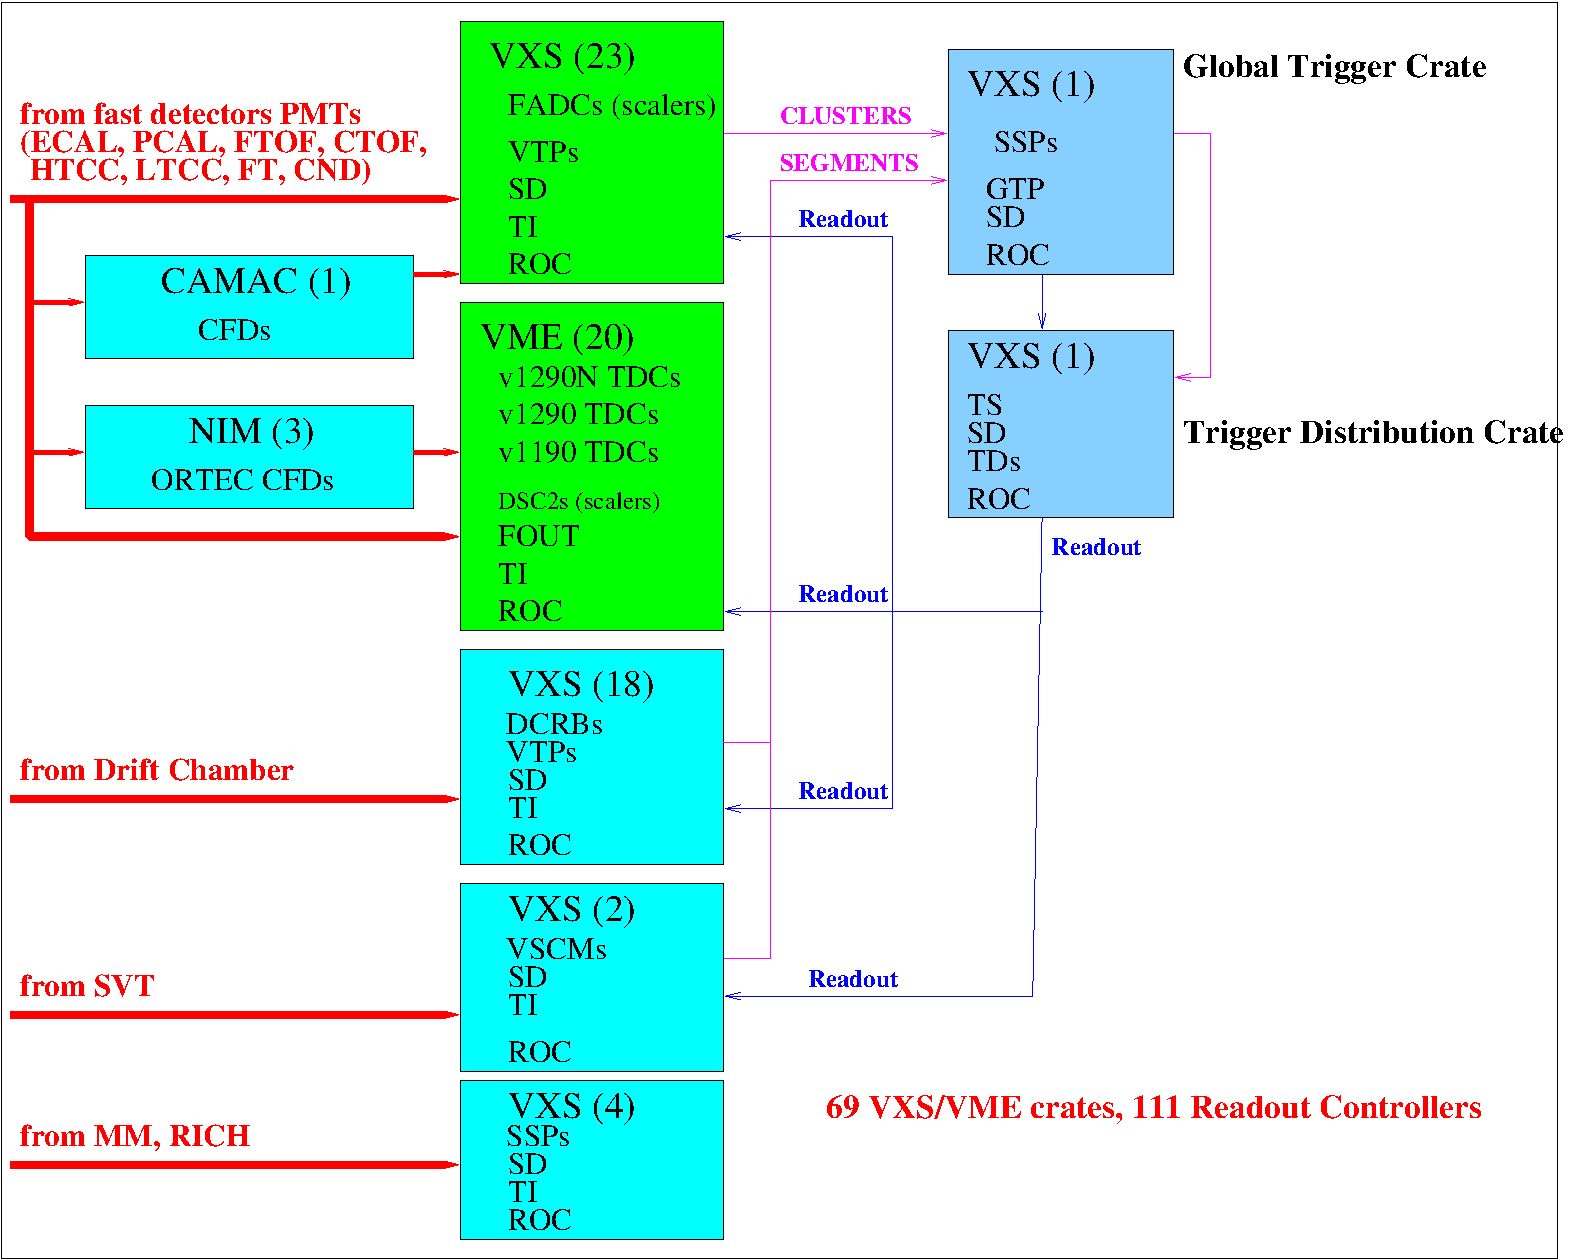
\includegraphics[width=1.0\columnwidth,keepaspectratio]{img/CLAS12_HARDWARE_2.pdf}
	\caption{CLAS12 Data Aquisition System Diagram}
	\label{fig:DAQdiagram}
\end{figure}


\section{Hardware Components}

New instrumentation modules have been designed by JLab that take advantage of the higher performance and elegant back-plane connectivity of the VITA 41 standard or ``VXS'', defined as VME with serial extensions. 
VXS was selected as the 12~GeV data acquisition back-plane foundation for the front-end detector readout and trigger hardware interface because this standard offered a method to easily synchronize and pass signals between each of the payload slots to a central switch fabric slot. At JLab a dual star back-plane configuration is used, and one switch slot is used for the trigger processing and one switch slot is used to distribute the essential timing and synchronization signals to each of the front-end boards.

The trigger processor switch slot board manages the high-speed gigabit signaling from each of the payload slots, where eight differential pairs connect from the payload slots to the switch slots. The VXS crates are manufactured by WIENER and the back-plane can support up to 8~Gb/s. The payload boards use Xilinx Virtex V technology, and these FPGAs have up to 6.25~Gbps transceivers. The payload boards are designed to run these high-speed gigabit transceivers at a maximum of 5~Gpbs to transfer trigger data to the trigger processor module. 

The design challenges for reliable and successful transmission of gigabit serial data over the VXS backplane requires the investment of high-speed circuit board layout and routing tools.  The FPGA selection requirements include at least four full duplex gigabit transceivers, user I/O pin count $>$~500, and fast integrated block memory with multi-rate FIFO logic. We use circuit board routing simulation tools such as Mentor Graphics HyperLynx [\ref], which are invaluable for critical simulation and verification of circuit board signal integrity for the gigabit transmission paths before the manufacturing process.  The FPGA devices that we use are capable of 6.25~Gb/s serial transfer, and we have designed our circuit boards with signal integrity techniques using standard FR4 circuit board material to achieve $>$~2.5~Gb/s, which meets the data transfer bandwidth requirements. 
Another significant investment required for the hardware verification of the gigabit transceivers was a digital signal analyzer with 8~GHz bandwidth to measure and record the backplane and fiber optic gigabit transceiver performance and to perform jitter analysis on the critical system clock and synchronization signals with at least 1~ps resolution.  We used the Tektronix jitter analysis software which is a critical tool for the verification of our system clock, and for measurements of the phase controlled jitter attenuated clock provided by the Signal Distribution (SD) switch card in every crate. The investment of firmware development tools from FPGA industry leaders Xilinx and Altera were also taken into consideration for the upgrade path to VXS. We use the Xilinx Aurora protocol for serial transmission as it is robust and simple, and is included with the FPGA development tools.  


\subsection{Fiber Optic Trigger distribution system}

As shown in Fig.~\ref{fig:hardwarediagram}, the digital sum value from each VTP in the front-end crate, and the distribution of the global clock, synchronization, and trigger commands from the global trigger hardware, use a separate fiber optic cable.  The crate sum fiber link is shown in orange, and the critical timing signals distributed to each front-end crate are blue.  Each fiber optic link makes use of the Avago POP4 fiber optic transceivers and parallel OM3-rated glass fiber cable with MTP connections. These fiber optic transceivers operate at 3.125~Gb/s for an aggregate bandwidth of 10 Gb/s which is ample enough for the summing information that is sent forward to the global trigger processing hardware.  The fiber link used for the distribution of the global clock, critical timing signals, and trigger commands runs at 1.25~Gb/s.

\begin{figure}[hbt]
	\centering
	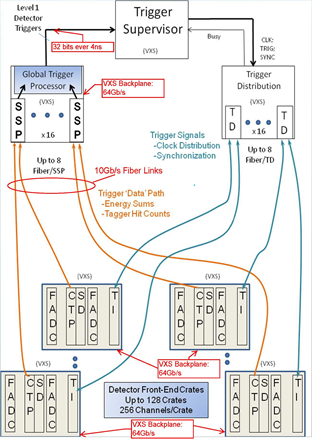
\includegraphics[width=1.0\columnwidth,keepaspectratio]{img/hardware_diagram.png}
	\caption{Hardware diagram with the implemented fiber links scheme.}
	\label{fig:hardwarediagram}
\end{figure}


\subsection{VXS/VME crates}

Previous experiments with the original CLAS spectrometer (see \cite{clas-nim}) used the VXI standard, which was a new extension of the original VME standard. VXI offered a method to distribute clock and other timing signals with low skews via the back-plane. 9U circuit boards were used that offered a large number of front panel input/output connections to handle the six sectors of the CLAS detectors that contributed to the level 1 trigger. The detector signals were acquired with FastBus ADC and TDC or in some instances, from VME or even CAMAC modules. 

During the initial design phase of the 12~GeV experiments the requirements of a 200~KHz sustained trigger rate demanded that the front-end modules adopt a new method of handling precision timing and synchronization over dozens of front-end crates. The latest technology at the 12~GeV inception included FPGA devices with high-speed serial transceivers built into the silicon fabric. A new VME extension was also emerging at the same time, which was labeled VXS, and defined a new high-speed gigabit connector with links between the VME slots and eight serial links to common switch slots. The VXS standard was declared as VITA 41 and several new standards have emerged in the past decade that expand the use of gigabit serial transmission via the crate back-plane. For the 12~GeV experiment era, we now have thousands of custom VXS payload and switch slot modules and hundreds of VXS front-end crates. Complex experiments and high channel count detectors make use of these custom VXS boards  designs for all four experimental halls at JLab.

\subsection{VME Crate Controllers}

The high-speed data physics acquistion and trigger systems for the JLab 12~GeV experiments have been standardized on the VME64X and VXS backplane and crate enclosure form-factor. In addition to the custom electronics that reside in these crates, there must also be a single ``controller'' for each crate. Considering all four experimental halls, this exceeds 100 controllers.

There are many commercial off-the-shelf options for this type of controller, and our general requirements do not extend beyond what is currently commercially available. We do have some specific requirements that narrowed the viable choices.

We purchased VME controllers from several vendors for development purposes and made a significant investment in custom software that runs on all of the existing boards. We also benchmarked our code and have come to expect certain ``minimum'' requirements for performance from the chosen architecture within an specified Linux operating system.

We also expect a certain minimum 10 year timeframe in which these controllers will be supported by the vendor with respect to the avilable parts, repair, and software updates. VME controller requirements are summerized in following list:

\begin{itemize}
	\item Single slot VME form-factor - no required rear transition module
	\item Intel Core i7 dual or quad core embedded processer 2~GHz (or greater)
	\item Hyperthreading and 64~bit arch support
	\item 4 GBytes DDR3 (1066~MHz) ECC SDRAM (or greater)
	\item Front panel gigabit ethernet and serial port console
	\item 1 x4 PCI Express XMC expansion slot (or greater)
	\item VME320-interface using the Tundra Tsi148 chip
	\item support for all VME transfer modes including 2eSST
	\item VXS optional: interface supporting both VITA 41.3 (Gig E) and 41.4 (PCIe) standards.
\end{itemize}

After several different boards were evaluated we purchased XVR16 Intel forth Generation 4-core i7-based rugged VME single board computers from GE (see Fig.~\ref{fig:XVR16diagram}). They were installed in the 70+ crates for CLAS12 and have demonstrated excellent performance and reliability. Most of the controllers send data over their built-in 1~GBit link, while for few of them, a 10~GBit daughter board was installed to increase the bandwidth. The maximum data rate from a single crate in CLAS12 never exceeds 130~MB/s, and with that rate 4-core controllers are able to handle the VME data polling, data processing, and sending data over the network without any issues. 

\begin{figure}[hbt]
	\centering
	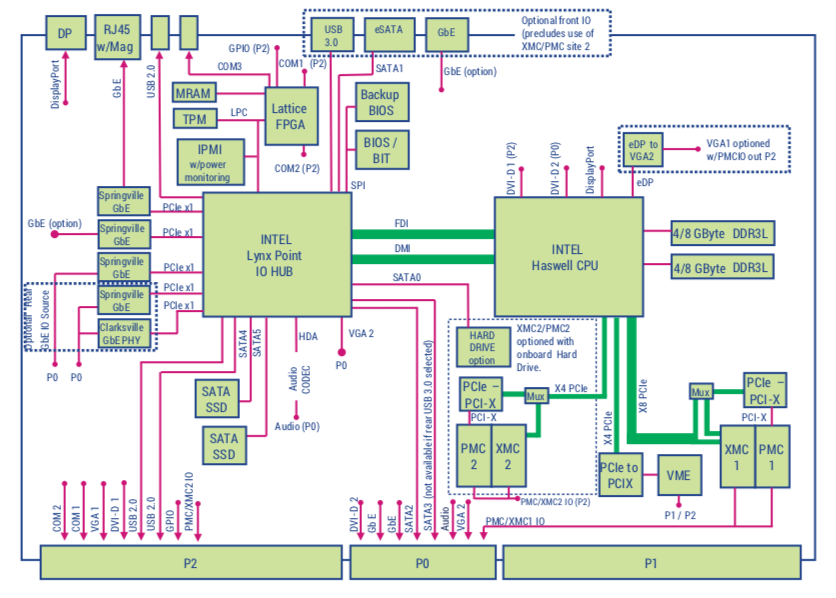
\includegraphics[width=1.0\columnwidth,keepaspectratio]{img/XVR16_diagram.png}
	\caption{Block diagram of the XVR16 VME crate controller}
	\label{fig:XVR16diagram}
\end{figure}



\subsection{Trigger Distribution System Modules (TS, TD, TI)}
	
The TCS (TRIGGER, CLOCK, SYNC, and BUSY) distribution system \cite{tcs-ref} is the hardware interface to bridge the trigger and the DAQ.  The TCS system receives the trigger decision from the trigger system, and initiates data readout for the DAQ system by distributing the readout trigger (TRIGGER) signal.  Additionally, it distributes a 250~MHz system clock (CLOCK) to pipeline the system, and it distributes an encoded synchronous signal (SYNC) for the system synchronization.  It monitors the frontend electronics’ status (BUSY) and makes sure of the smooth data readout of the experiments. Fig.~\ref{fig:TCSdiagram} shows a diagram of the trigger and TCS distribution.

\begin{figure}[hbt]
	\centering
	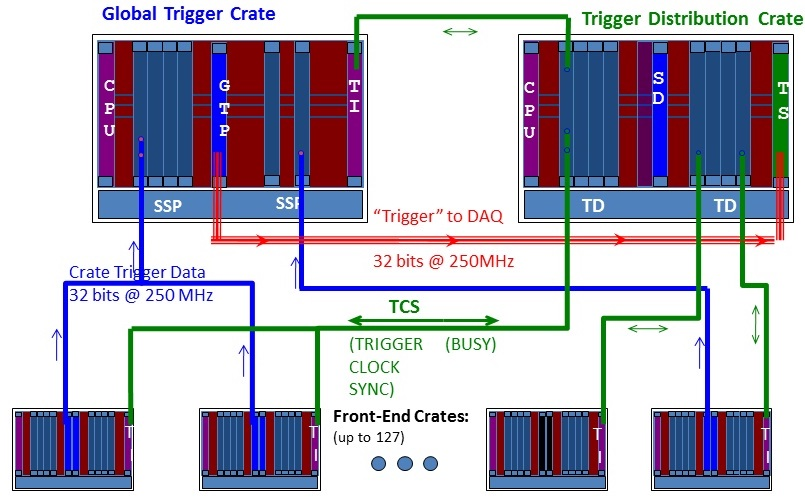
\includegraphics[width=1.0\columnwidth,keepaspectratio]{img/TCSdiagram.jpg}
	\caption{Diagram of the trigger and TCS distribution. The VTP boards generate triggers using detector signals from the front end crates.  The final trigger decisions, up to 32 trigger types, are sent from VTP to TS for data readout.  The TS distributes the TCS to the TD through SD and the backplane, then to the front end crate through optic fiber and TI.  The TI collects the front end boards busy signals and sends to TD, then throttle (disable) the readout trigger distribution on TS.
}
	\label{fig:TCSdiagram}
\end{figure}


The main hardware of the TCS distribution system includes a Trigger Supervisor (TS \cite{ts-ref}) board (see Fig.~\ref{fig:TSused} and ~\ref{fig:TSdiagram}), Signal Distribution (SD \cite{sd-ref}) boards, Trigger Distribution (TD \cite{td-ref}) boards  (see Fig.~\ref{fig:TDused}), Trigger Interface (TI \cite{ti-ref}) boards  (see Fig.~\ref{fig:TIused} and ~\ref{fig:TIdiagram}), VXS crates, and optic fibers.  The TS board, one SD board, and up to sixteen TD boards are located in the global TCS distribution VXS crate.  One TI board and one SD board and/or one FANIO board are located in each front-end crate.  The electronics boards were custom designed and produced for the 12 GeV upgrade.  Field Programmable Gate Arrays (FPGA) are used for TCS generation, control, and decoding.  Optical fibers and high-speed differential backplane connections are used to transmit signals at high speed over long distances.  

\begin{figure}[hbt]
	\centering
	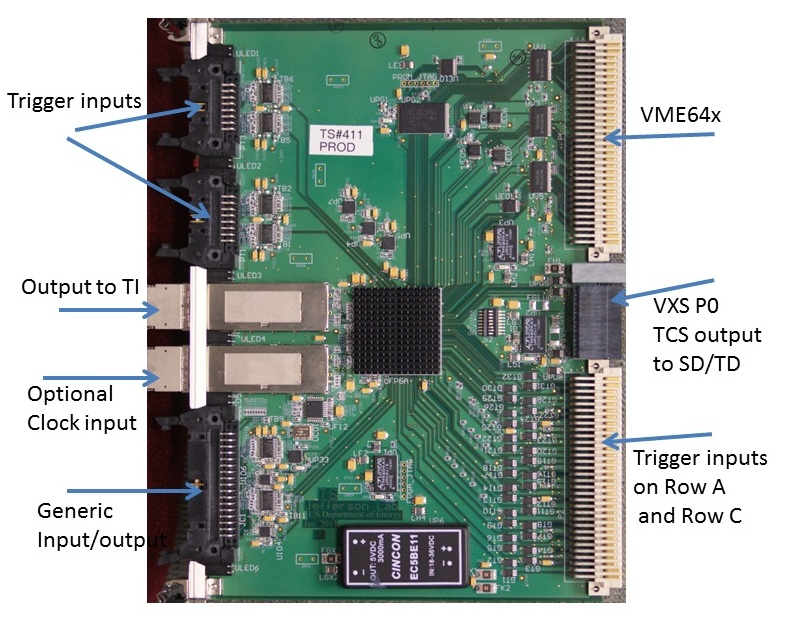
\includegraphics[width=1.0\columnwidth,keepaspectratio]{img/TSused.jpg}
	\caption{Trigger Supervisor (TS) board.  The TS board is a 6U by 160mm VME board with VXS connector.  It generates and distributes the readout triggers, synchronization signals, and clock (either from the front panel input or the on-board oscillator) to the TD boards via the SD through the VXS backplane.}
	\label{fig:TSused}
\end{figure}

\begin{figure}[hbt]
	\centering
	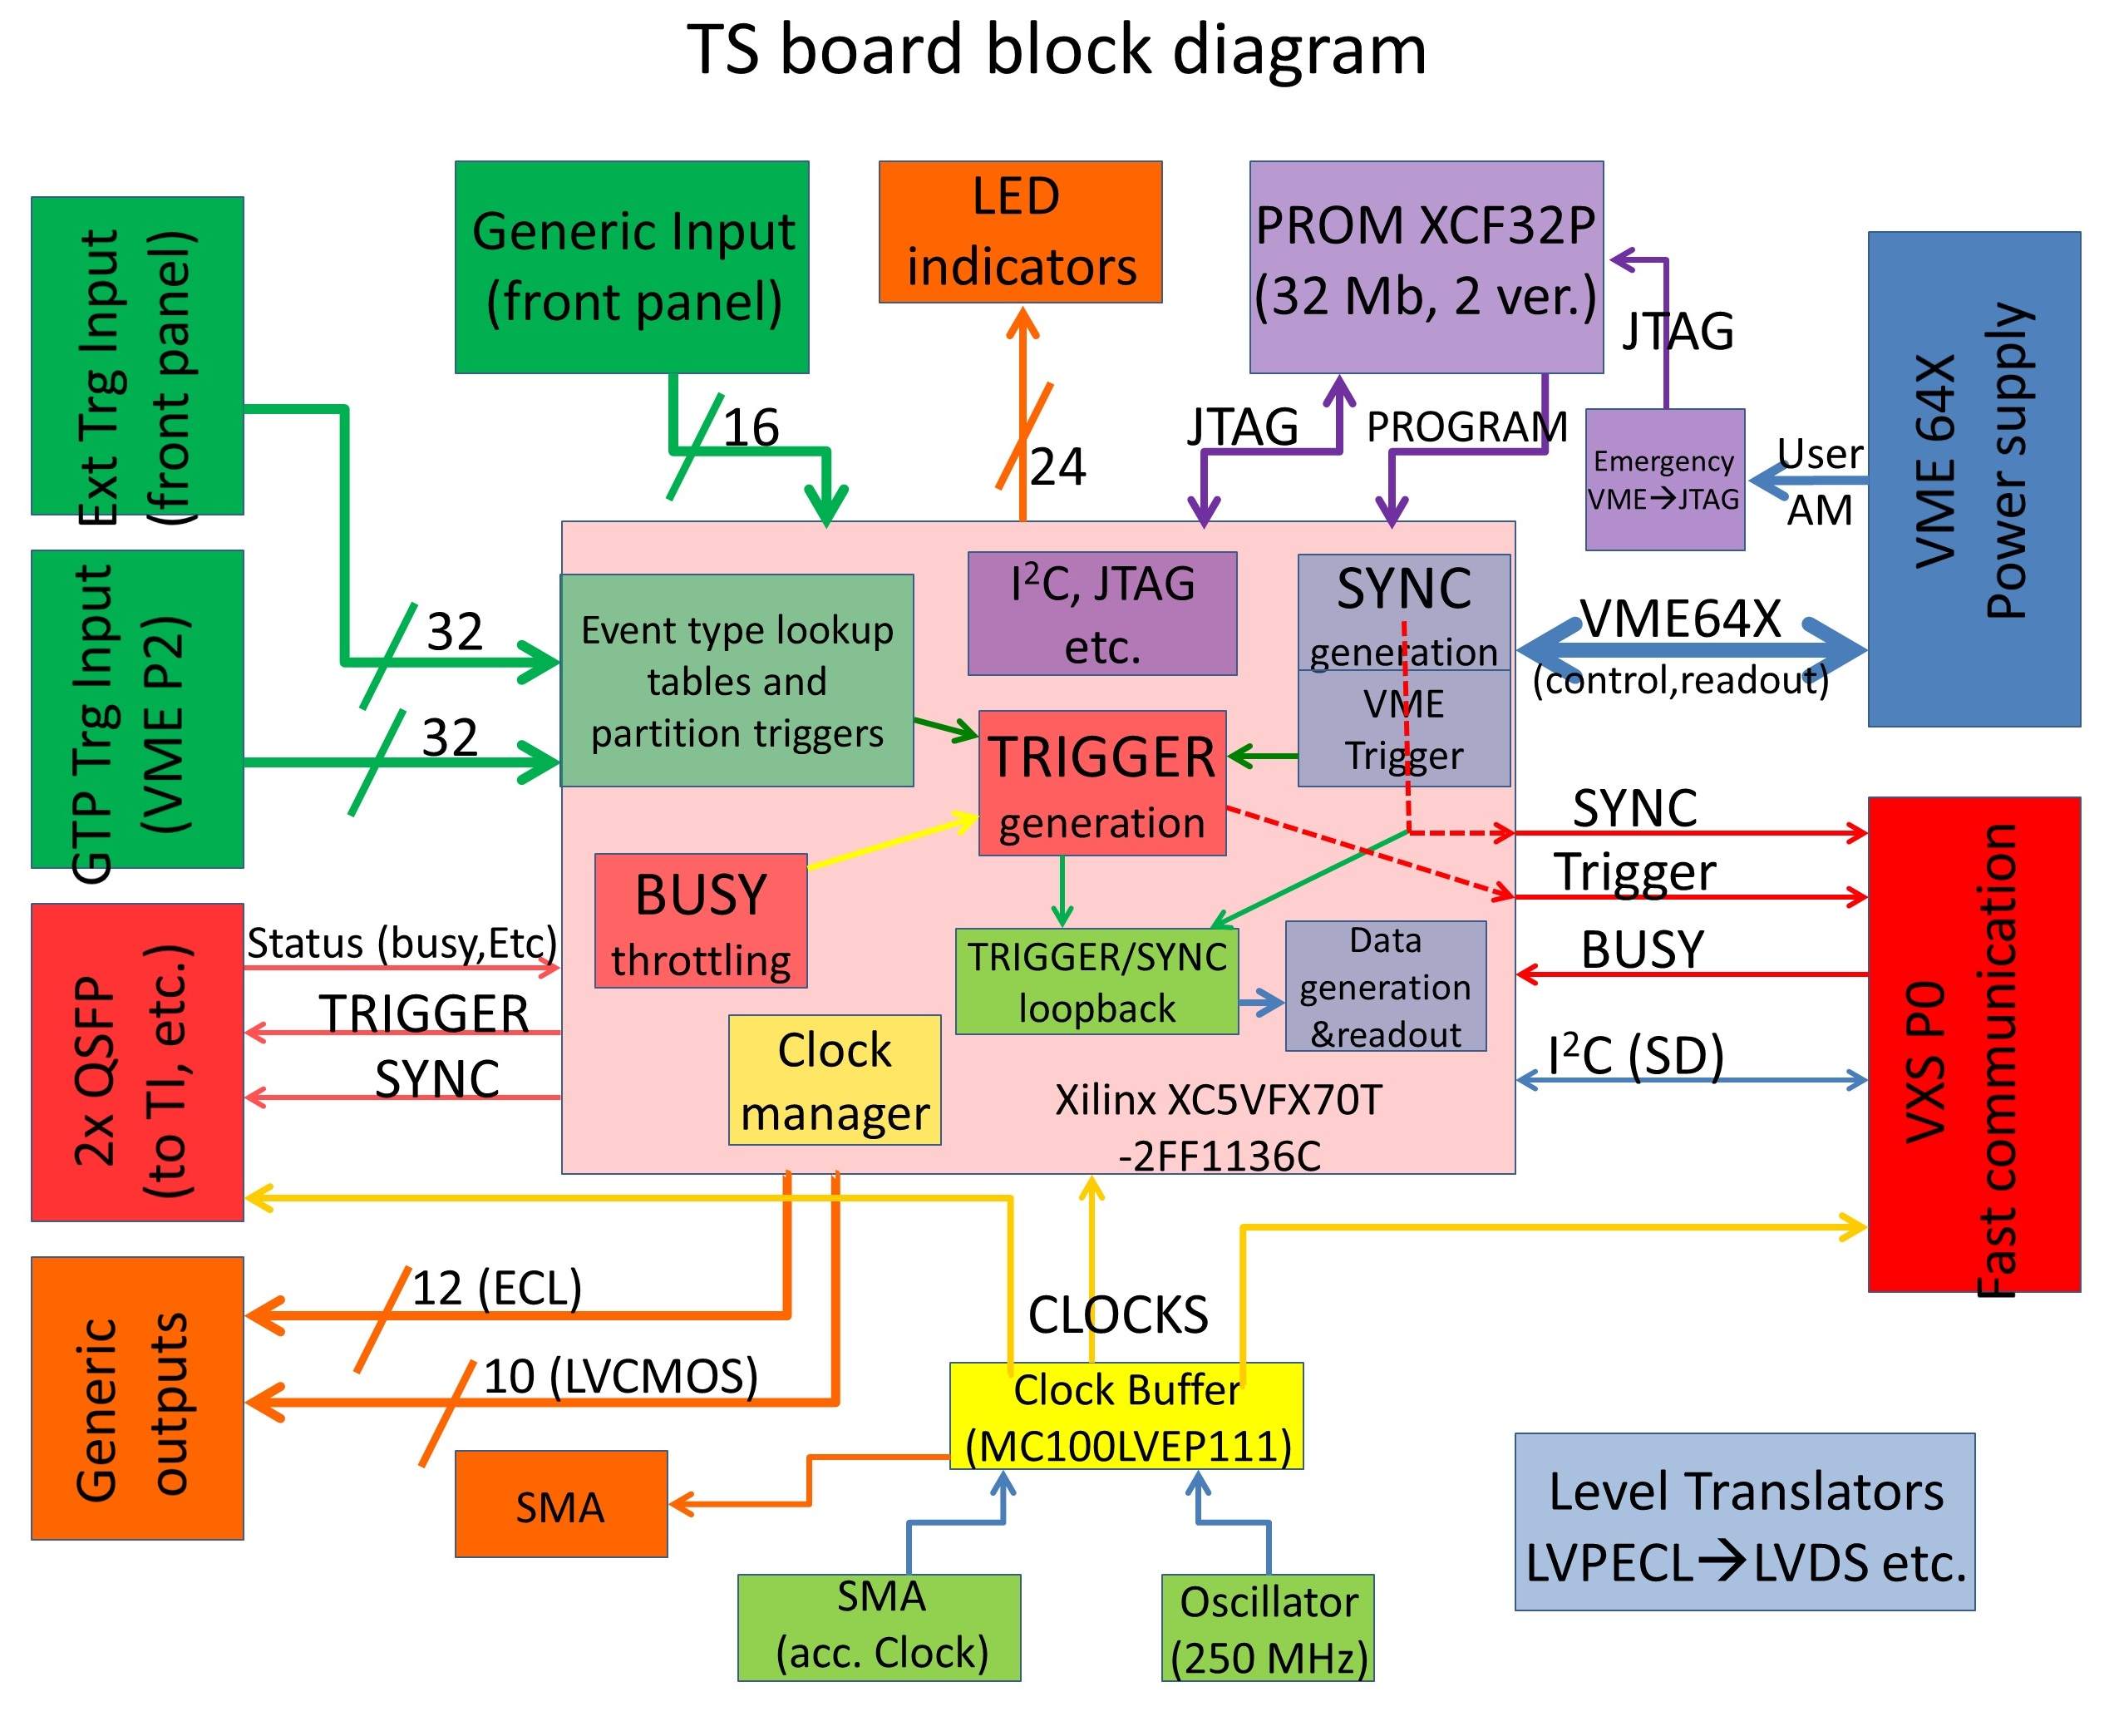
\includegraphics[width=1.0\columnwidth,keepaspectratio]{img/TSdiagram.jpg}
	\caption{TS board diagram.  The TS generates the readout triggers from up to 32 front panel trigger inputs and up to 32 backplane trigger inputs (from GTP), and sends out the triggers via encoded 16-bit words to the backplane.}
	\label{fig:TSdiagram}
\end{figure}

\begin{figure}[hbt]
	\centering
	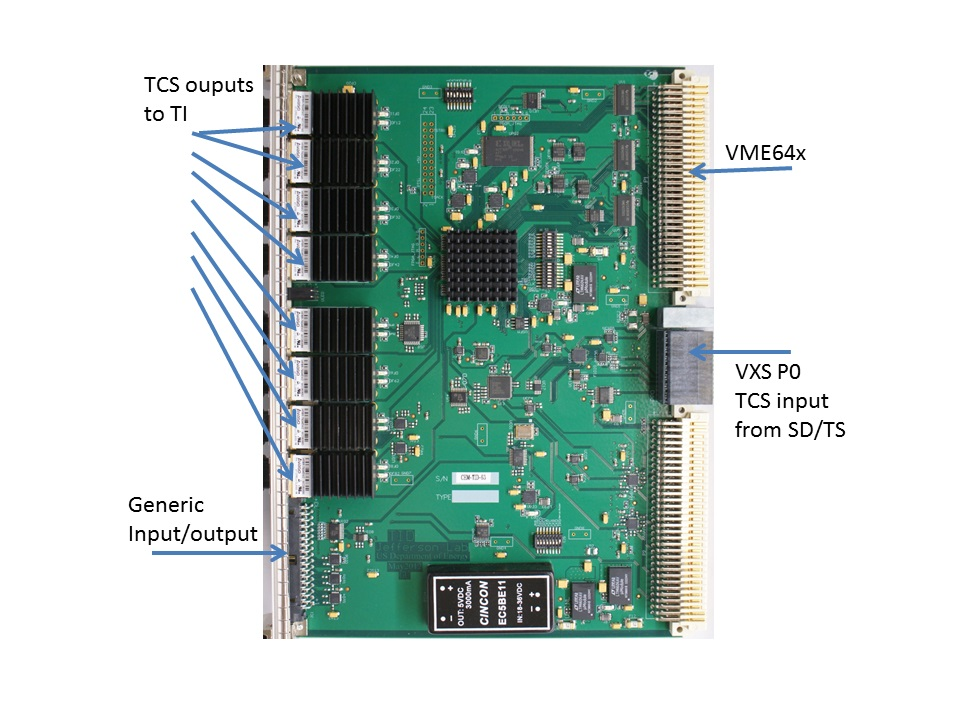
\includegraphics[width=1.0\columnwidth,keepaspectratio]{img/TDused.jpg}
	\caption{Trigger Distribution (TD) board.  The TD board is a 6U by 160mm VME board with VXS connector.  It receives the TCS from TS via the VXS backplane, and distributes the TCS via the front panel QSFP optic links.  It collects the Busy inputs from up to eight TI boards, and generates the readout buffer busies for up to eight front end crates.  The TD sends the collective BUSY to TS to back pressure the trigger generation.}
	\label{fig:TDused}
\end{figure}

\begin{figure}[hbt]
	\centering
	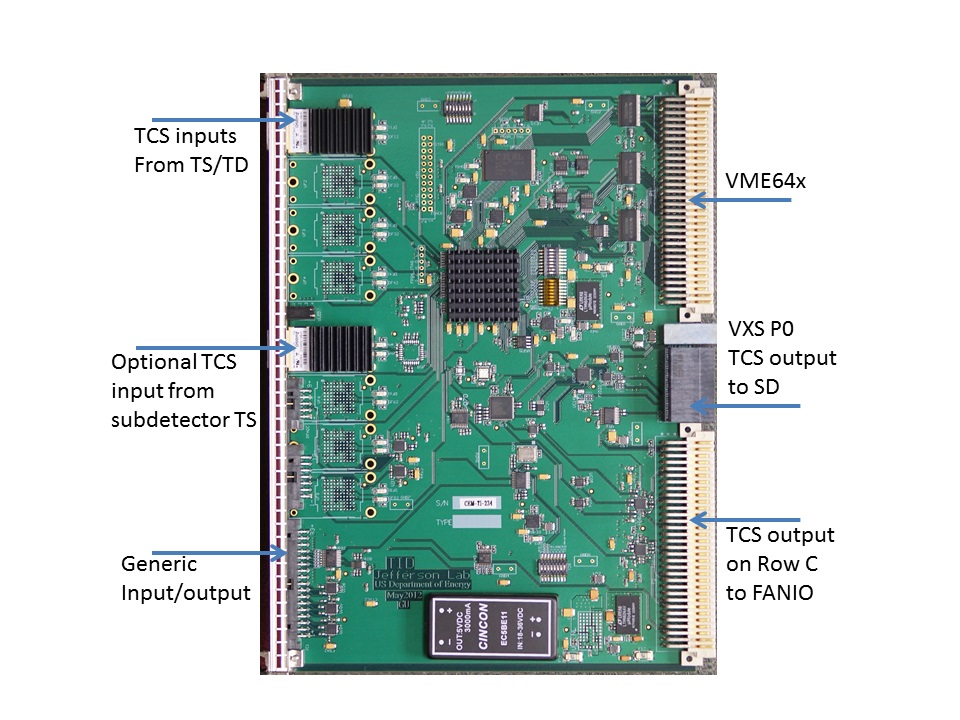
\includegraphics[width=1.0\columnwidth,keepaspectratio]{img/TIused.jpg}
	\caption{Trigger Interface (TI) board.  The TI board is a 6U by 160 mm VME board with (or without) the VXS connector.  It is using the same PCB as TD board with modified components population.  It receives the TCS from TS/TD or a sub-system controller via fiber, and collects the busy and sends to TS/TD via the same fiber.  The TI can also be used as a subsystem controller in the so-called master mode.}
	\label{fig:TIused}
\end{figure}

\begin{figure}[hbt]
	\centering
	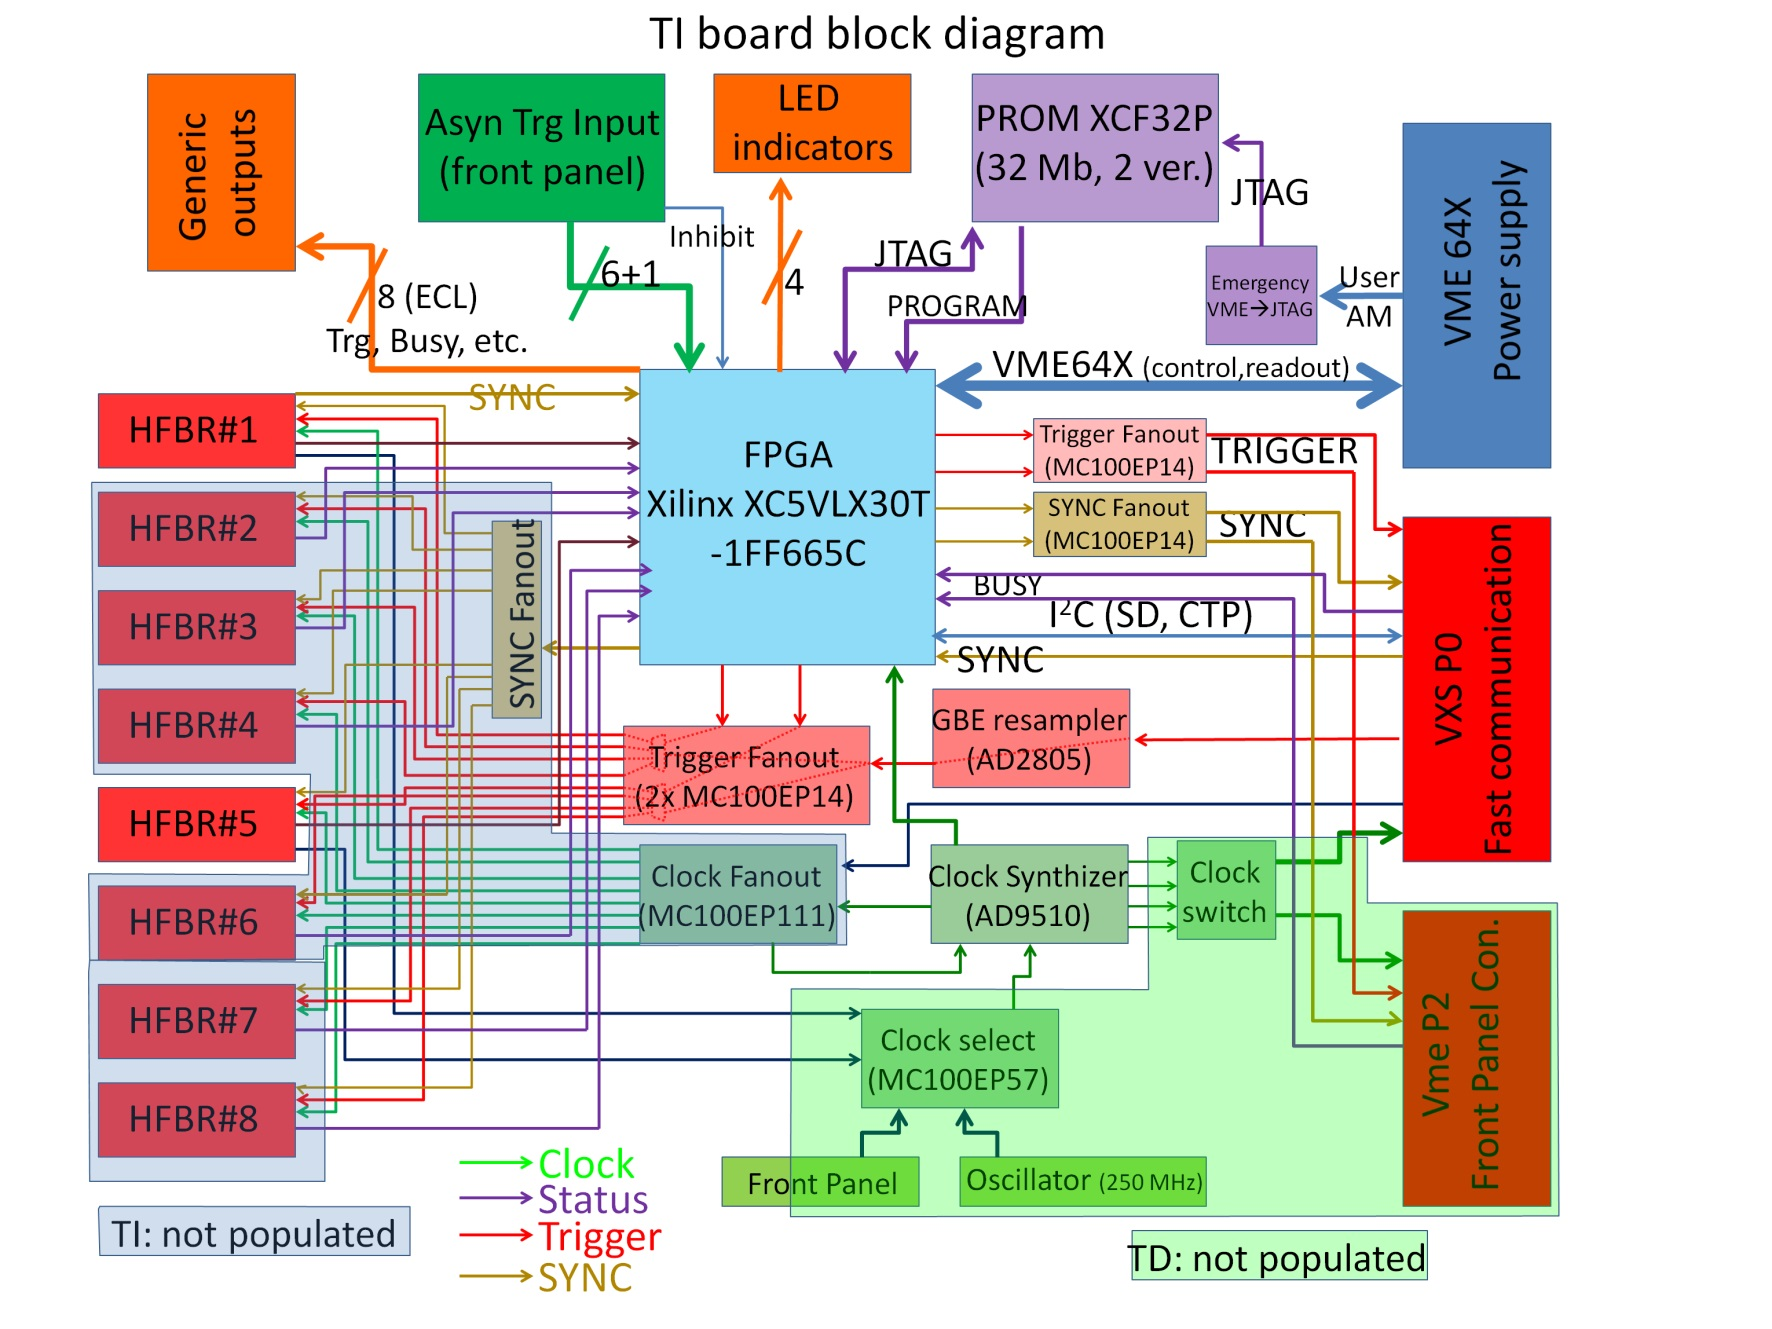
\includegraphics[width=1.0\columnwidth,keepaspectratio]{img/TIdiagram.jpg}
	\caption{TI and TD board diagram.  The TI and TD use the same PCB design, but different component population and FPGA firmware.}
	\label{fig:TIdiagram}
\end{figure}


\subsubsection{Clock Distribution}

The TCS system uses the 250 MHz clock, that comes from the TS in the global trigger distribution crate.  This clock is either generated by the TS on-board oscillator or its fronts panel input.  The clock is fanned out to the VXS P0 connector and then to the SD board.  The SD fans out the clock to the TD boards via the VXS P0 backplane.  The TD boards further fan out to the TI boards via optic fibers.  The TI uses this clock to generate clocks with proper frequencies (250 MHz, 125 MHz, 62.5 MHz, 31.25 MHz and 41.67 MHz) and sends the clocks to the front-end crate SD board, and the SD fans out to the front-end DAQ modules (TDC, ADC).  The fan-out buffer level is minimized on every board to limit the clock jitter.  The slower clocks derived from the main system clock are phase aligned thanks to the Analog Devices AD9510 with a synchronous phase re-alignment command.  The clock jitter is about one ps measured at the front-end electronics.  The clock distribution skew can be adjusted by the SD clock delay if necessary.


\subsubsection{SYNC Distribution}

The TS generates and distributes the SYNC signal.  The SYNC is an encoded 4-bit serialized command transferred at 250 Mbps synchronized with the system clock.  Normally, the serial SYNC line stays at logic high (or ‘1’).  When transferring a SYNC command, the SYNC goes to logic low for one bit, followed by the 4-bit command code.  After the 4-bit SYNC command, the SYNC goes to logic high again.  There is a minimum of four ‘1’s before the next cycle begins.  The SYNC start is phase aligned to the 62.5 MHz clock used for the trigger word transfer, the 41.67 MHz clock used for the CAEN TDC boards, and the 31.25 MHz clock used for Flash ADC boards.  This phase relation is used to synchronize the slower clocks on the TI to the 62.5 MHz clock on the TS.  This also limits the SYNC command to no more than one per 96 ns.  To facilitate the AC coupled optical transceivers, the SYNC is Manchester encoded on the TS and the TD, and Manchester decoded on the TI and the TD.

The SYNC is phase aligned with the 250 MHz system clock on the TI boards using their FPGA’s IODELAY.  The SYNC is synchronized across the TI boards by applying different delays on the individual TI boards.  The delays are determined by the fiber latency measurement.  

The spare fibers between the TD and TI boards are used to measure the fiber latency.  The TI sends a test signal to the TD through one fiber, and the TD loops back the signal through another fiber.  The TI measures the delay between the test pulse and the looped back test pulse using the FPGA counter and the carry chain in the FPGA.  As the fiber skew is small (less than 1 ns for 100 meter fibres), the measurement on these two fibres can be used as the latency of the other fibres in the cable.  
After the SYNC latency compensation, all the TI boards receive the SYNC at the same time with the skew of one system clock period, which is 4 ns.  The synchronized SYNC signals are used to synchronize the triggers as described next.


\subsubsection{Trigger Distribution}

The trigger words, which include the readout trigger signals and event information (event type, trigger timing, etc.), are generated and serialized on the TS.  The serialized trigger word is fanned out by the SD board and the TD board, and deserialized by the TI board.  The 16-bit trigger words are summarized in Table~\ref{tab:trigger_word_definition}.  

\begin{table}
\begin{adjustbox}{width=\columnwidth,center}
	\begin{tabular}{| l | l | l | l |}
		\hline \hline
		Bit 15:12		& 	Bit 11:10 &	Bit 9-0	 & Comment		\\
		\hline
	1001	& Quadrant timing	& Event type	 & GTP major trigger \\
	1010	& Quadrant timing	& Event type	 & Ext major trigger \\
	
	1011	& \multicolumn{2}{c}{Four TS partitions’ event types}    & TS partitioning (4, 3, 2, 1) \\

	\multirow{2}{*}{0110}	& \multirow{2}{*}{Quadrant timing}	& Trigger source & TImaster legacy Trigger \\
		    &                   & Event type	 & (TS) VME trigger     \\
	0101	& Trigger command/Control	& VME command \\
	0100	& TS timer (TS time bit(13:2))	& TI Sync check \\
	0111	& Trigger content	& Additional trigger info \\
		\hline \hline
	\end{tabular}
\end{adjustbox}
\caption{Trigger word definition.  The TS encode the readout trigger, event type, and the fine timing (4ns quadrant) information into a 16-bit word, which is transferred every 16ns.  This 16-bit word can also be some system setting information or the system timer when there is no readout trigger in the 16ns periods.}
\label{tab:trigger_word_definition.}
\end{table}

Both the fiber latency and trigger word serializer/ deserializer are compensated so that all the TI boards send the readout trigger at the same time to the front-end data acquisition electronics.  The SYNC is used in conjunction with a synchronous FIFO to enforce a fixed latency on the trigger distribution. Fig.~\ref{fig:TIsync} shows the diagram of the compensated trigger distribution.

\begin{figure}[hbt]
	\centering
	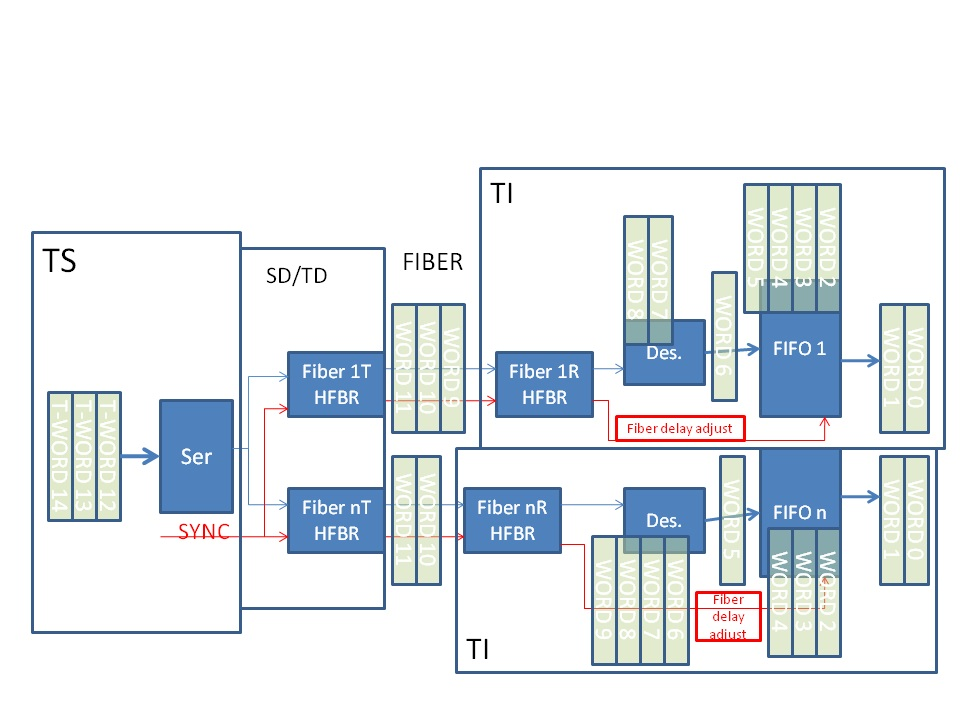
\includegraphics[width=1.0\columnwidth,keepaspectratio]{img/TrgSync.jpg}
	\caption{Trigger synchronization between TIs.  The TI boards delay the decoding of the received readout trigger by the complement of the TS/TD to TI transfer latency, so that all the front end boards receive the readout trigger simultaneously.}
	\label{fig:TIsync}
\end{figure}

On the TI board, the deserialized trigger word is clocked into and clocked out of a FIFO using the 62.5~MHz clock.  At the start-up, the FIFO is reset (0 words) and the FIFO read/write is disabled.  The serial trigger link is idle words only.  On trigger start, the TS starts trigger word transmission.  The TI will write the deserialized data (valid data, that is non-idle data word) to the FIFO.  After some pre-set delay (VME register controlled), the TS issues a ‘Trigger Start’ command on the SYNC link.  When TI receives the ‘Trigger Start’, the TI resets the trigger FIFO readout address, and enables continuous readout of the FIFO.  As the SYNC lines are fiber length adjusted and the 62.5 MHz clocks are phase aligned, the trigger words from the TI board FIFO are synchronized across the system.
The trigger word also has the fine trigger timing information.  By decoding that, the TI board distributes the trigger in 4 ns precision, although the trigger word is serialized every 16 ns.  If the system clock phase is not adjusted, there will be a maximum of 4 ns skew among the clocks on the TI boards, so does the readout trigger.  The clock phase can be adjusted by SD if the skew is critical to the system.


\subsubsection{DAQ synchronization (trigger throttling) control}

Because of the finite memory size and the randomness of the triggers, it is possible for the memory to become overwhelmed somewhere in the system, which could cause DAQ problems.   The TCS throttling mechanism is used to prevent possible memory overflows, and to keep the DAQ synchronized.  Fig.~\ref{fig:DAQ_synchronization} shows the DAQ synchronization logic implementation.  Three methods are used to keep the DAQ synchronized.  These include trigger rules and event limit setting, pipeline DAQ, and synchronization events (special events).

\begin{figure}[hbt]
	\centering
	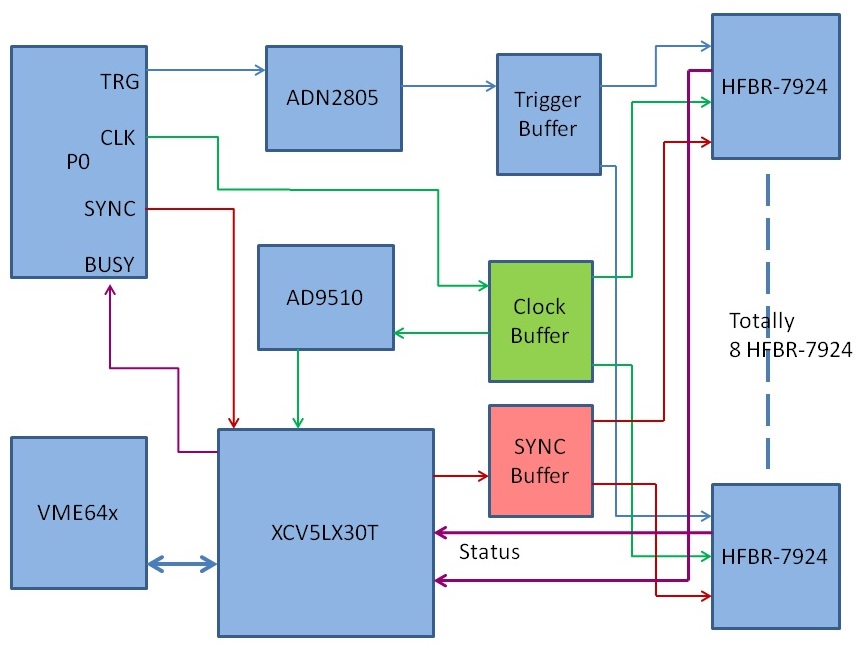
\includegraphics[width=1.0\columnwidth,keepaspectratio]{img/TDdiagram.jpg}
	\caption{DAQ synchronization}
	\label{fig:DAQ_synchronization}
\end{figure}


%REFERENCES
%[1] 	J. Gu etal. (2014, May). The TRIGGER/CLOCK/SYNC Distribution for TJNAF 12 GeV Upgrade Experiments    %https://coda.jlab.org/wiki/index.php/Trigger_distribution_overview
% [2] 	J. Gu. Description and technical information for the Trigger Supervisor (TS) module.  TJNAF, VA, 2013.  %Available: https://coda.jlab.org/drupal/system/files/pdfs/HardwareManual/TS/TS.pdf 
%[3] J. Gu, etal, 	“Design of the Trigger Interface and Distribution Board for TJNAF 12 GeV Upgrade,” IEEE Trans. Nucl. %Sci., Vol. 60, no. 5, pp 3714-3719, Oct. 2013

	
\subsection{Signal Distribution Module (SD)}

The Signal Distribution Board (SD \cite{sd-ref}) module (see Fig.~\ref{fig:SDpic}) occupies the “B” switch card slot as specified in VITA 41. The main purpose of this module is to distribute the signals received from payload slot 18 (Trigger Interface board) of a VXS crate to the 16 other payload slots (ADC boards).

The SD module distributes the 4 LVPECL differential pair  signals from payload slot 18 to 16 VXS payload slots within the crate. This is done using the high-speed, point-to-point connections from the switch slot to each payload slot. The four distributed signals are length-matched to minimize the output jitter seen on all of the payload slots. Three of the four remaining pairs are LVDS signals routed from the each payload module to the FPGA on the SD module. The last pair is an LVDS signal routed from the FPGA on the SD module to each payload module. Each of the 16 payload modules has a single-ended signal to the SD module and one from the SD module back to the payload module.

\begin{figure}[hbt]
	\centering
	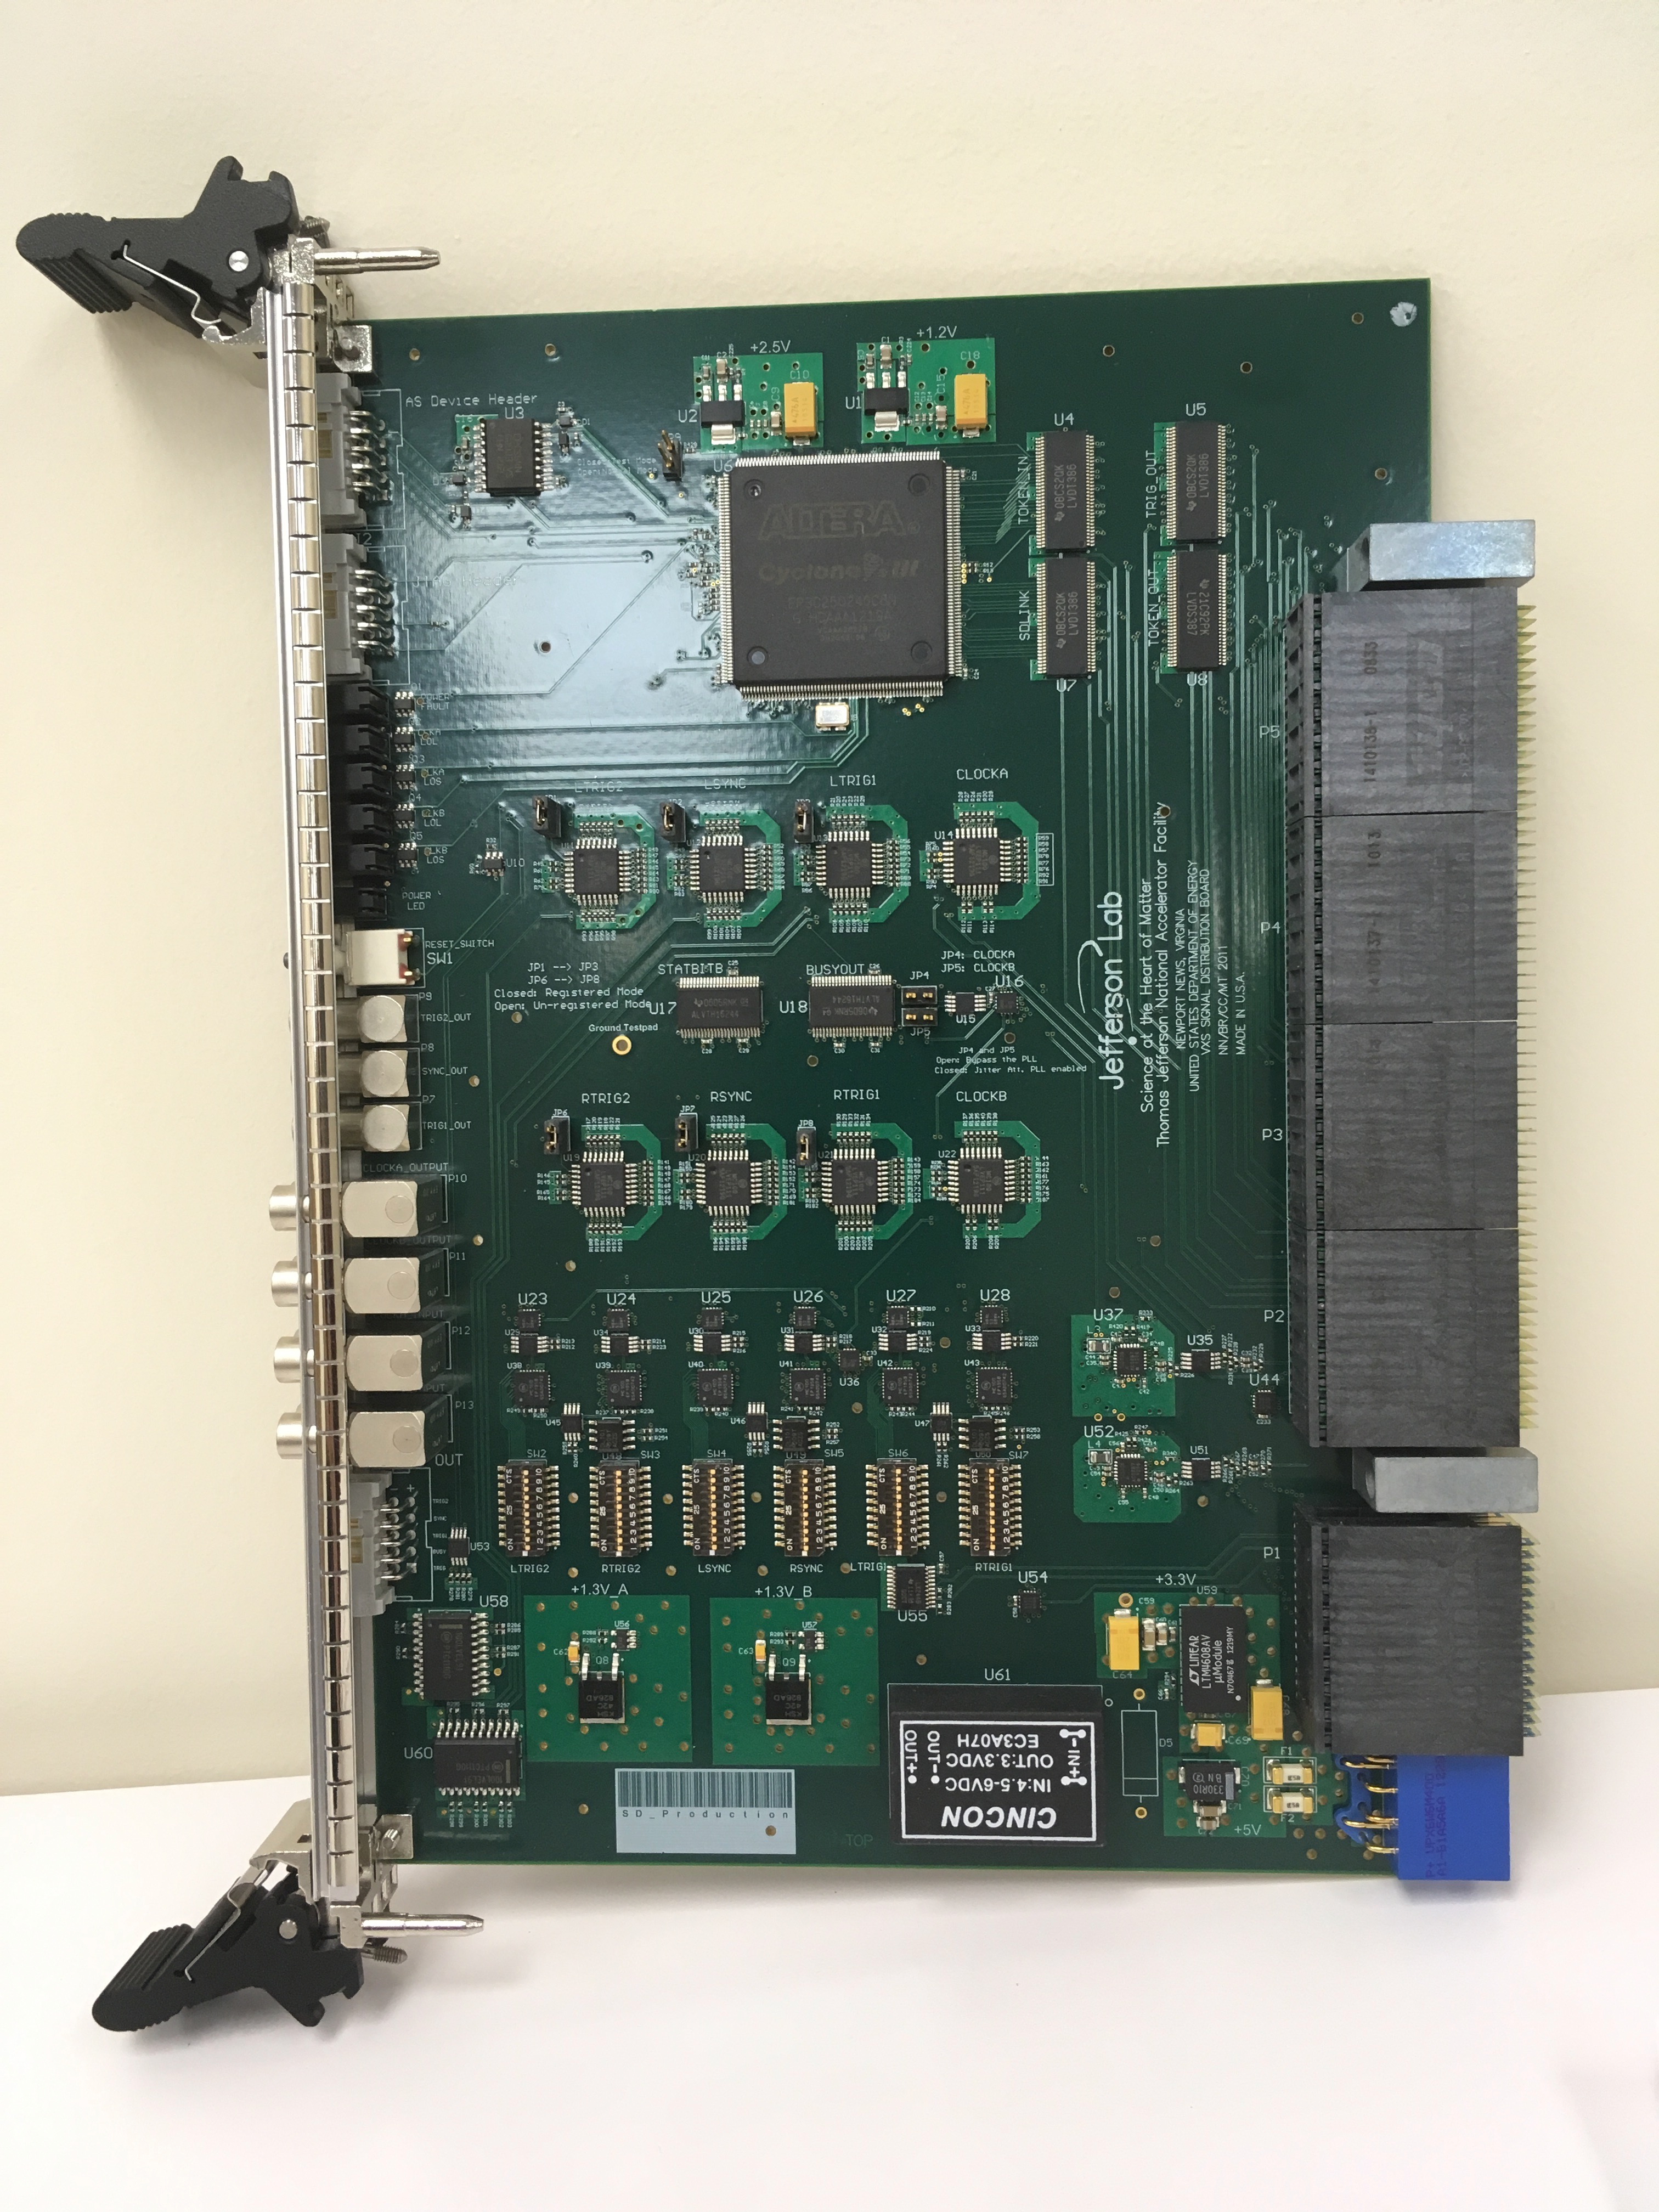
\includegraphics[width=1.0\columnwidth,keepaspectratio]{img/sd_board.jpg}
	\caption{Signal Distribution module (SD)}
	\label{fig:SDpic}
\end{figure}


\subsection{Flash ADC Module (FADC250)}

A 16-channel 250 MSPS pipelined flash ADC (FADC \cite{fadc-ref}, see Fig.~\ref{fig:FADC250pic}) with 12-bit precision was designed to digitize and process detector pulses for experiments at JLab.  The FADC250 module (see Fig.~\ref{fig:FADC250_board}) conforms to the VITA-41 VME64x switched serial (VXS) standard.  Each channel of the module accepts input signals on a LEMO style coaxial connector and has three user-selectable ranges (0.5 V, 1.0 V, 2.0 V).  Differential signal conditioning scales the input signals to within the dynamic range of the ADC and a single-pole low pass filter limits the signal bandwidth to the Nyquist band of the converter (125 MHz). Individual channel offsets are accomplished by means of DACs under VME control.  Each channel has its own dedicated ADC chip (Analog Devices AD9230). Both positive and negative polarity input signals are supported. The 250 MHz clock is distributed to the ADC chips through a low jitter ($<$ 2~ps) network.  

\begin{figure}[hbt]
	\centering
	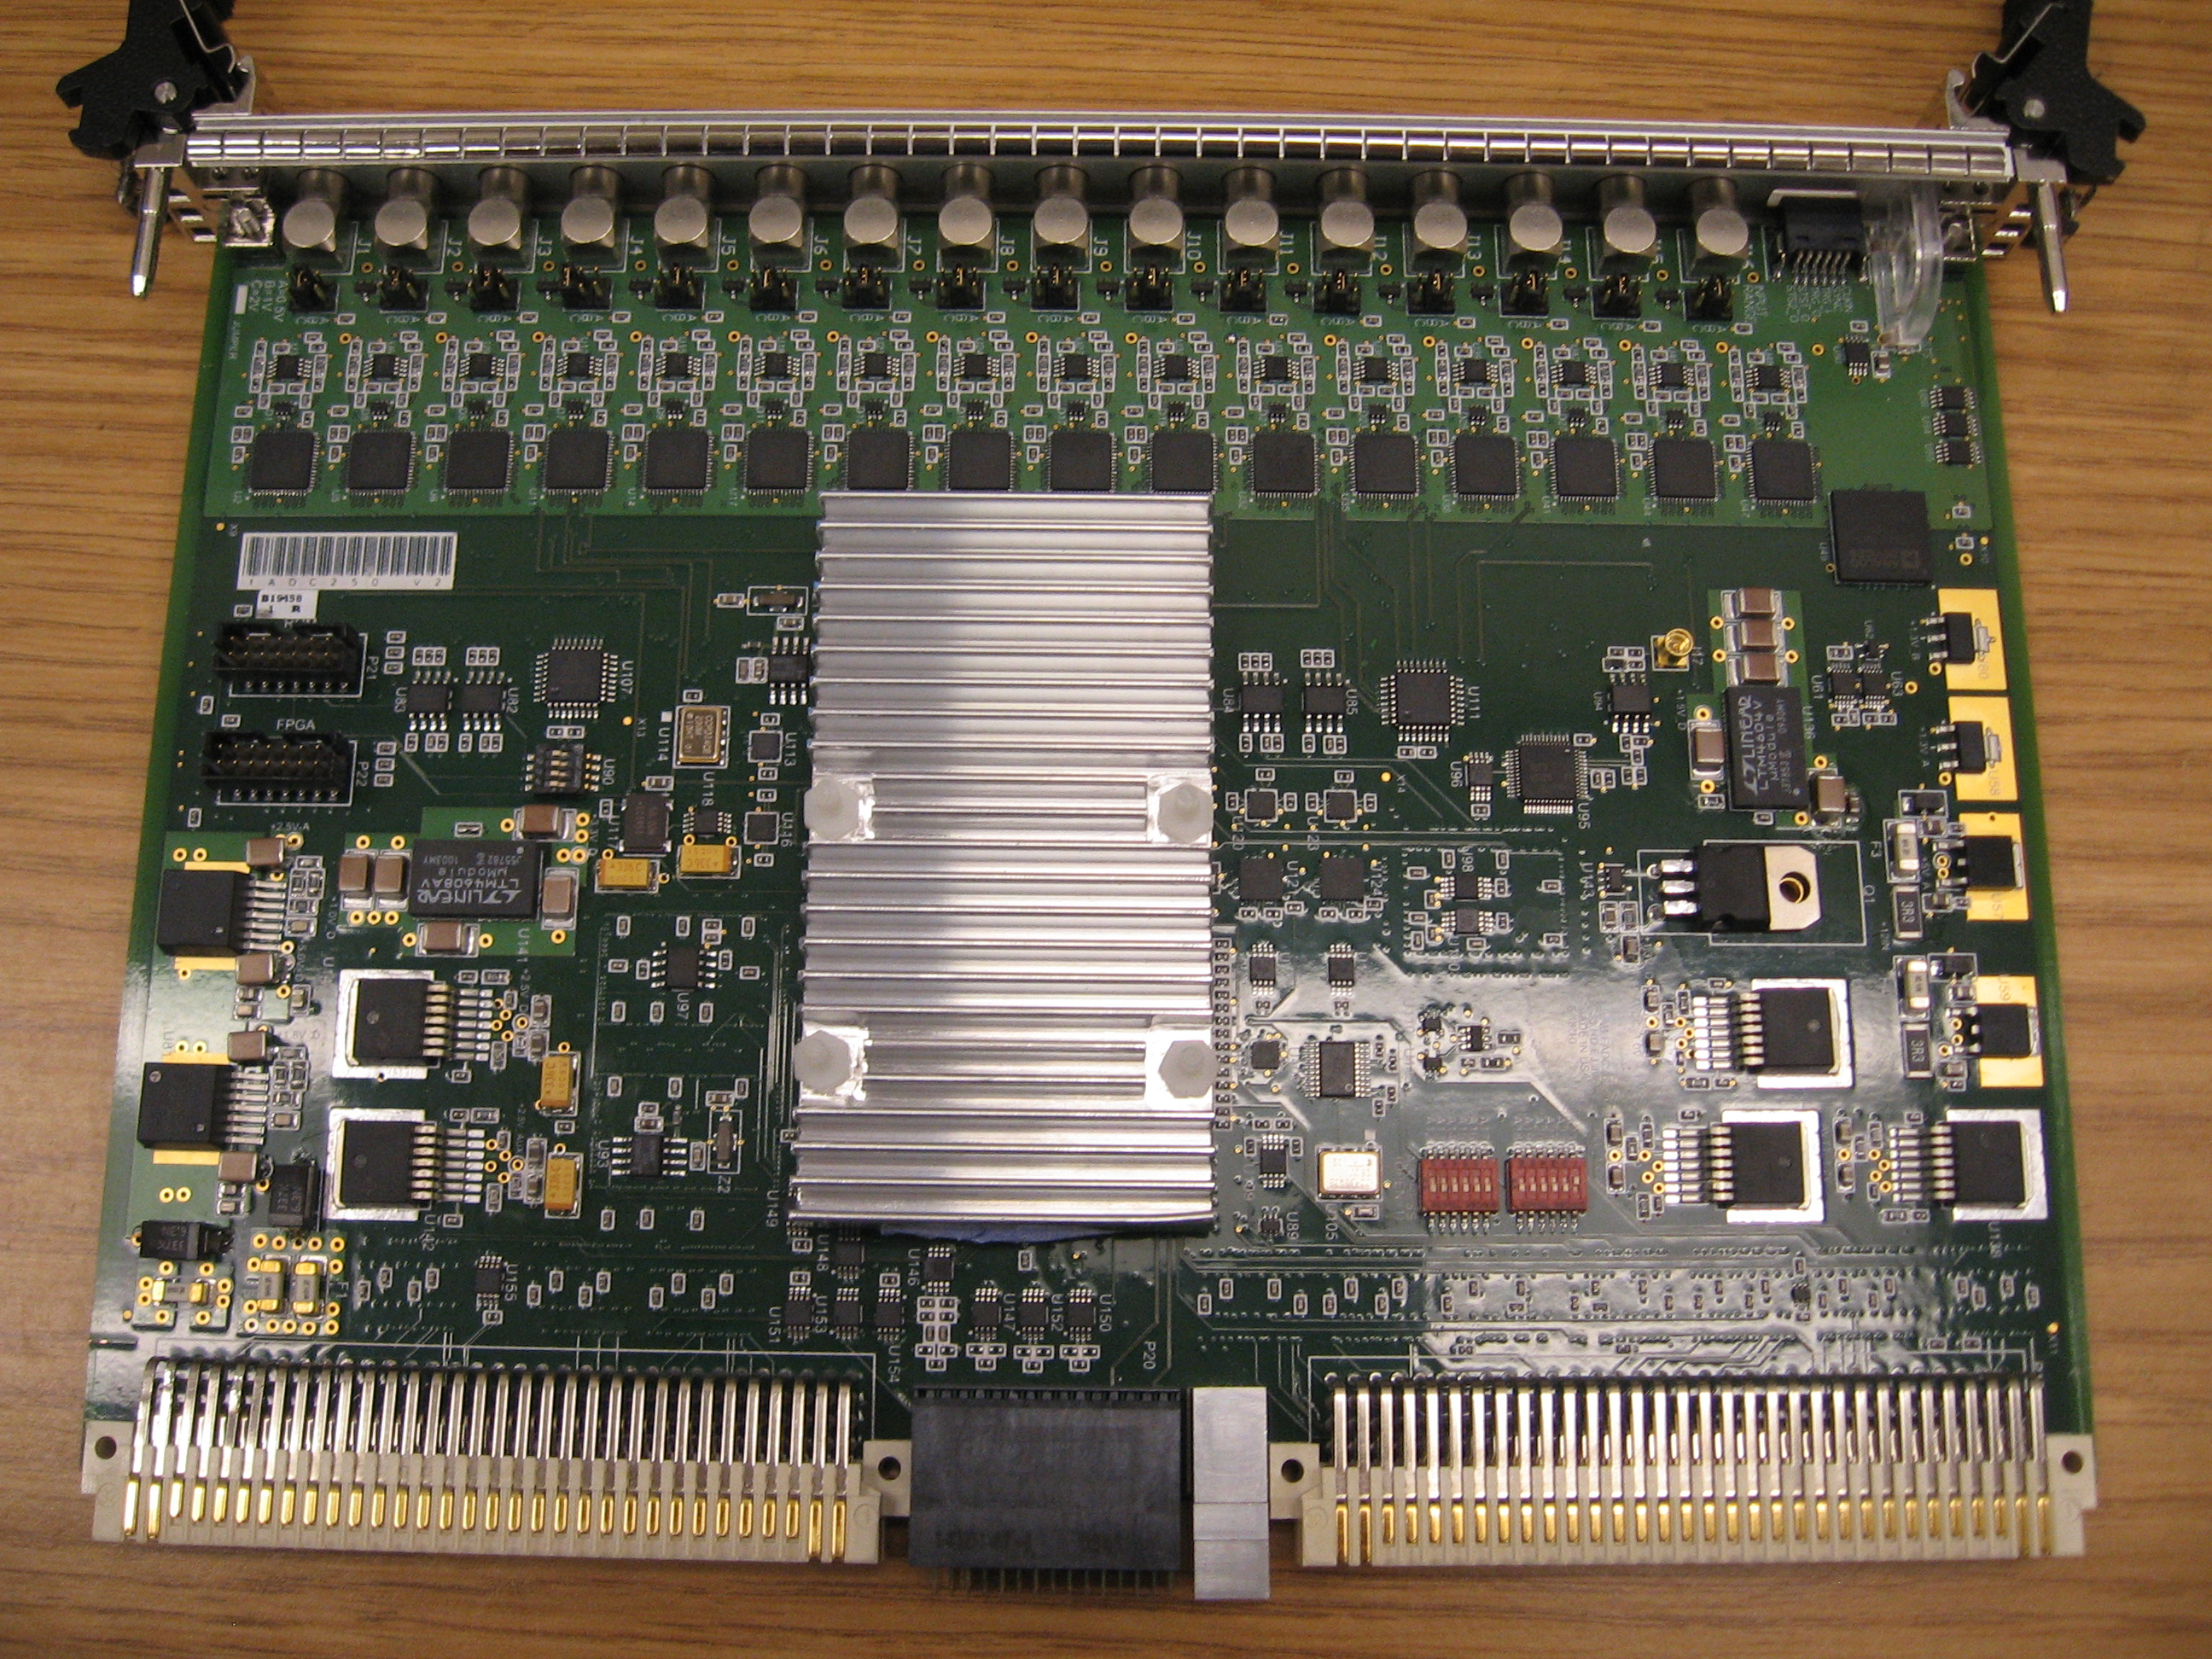
\includegraphics[width=1.0\columnwidth,keepaspectratio]{img/FADC250pic.jpg}
	\caption{Flash ADC module (FADC250)}
	\label{fig:FADC250pic}
\end{figure}

\begin{figure}[hbt]
	\centering
	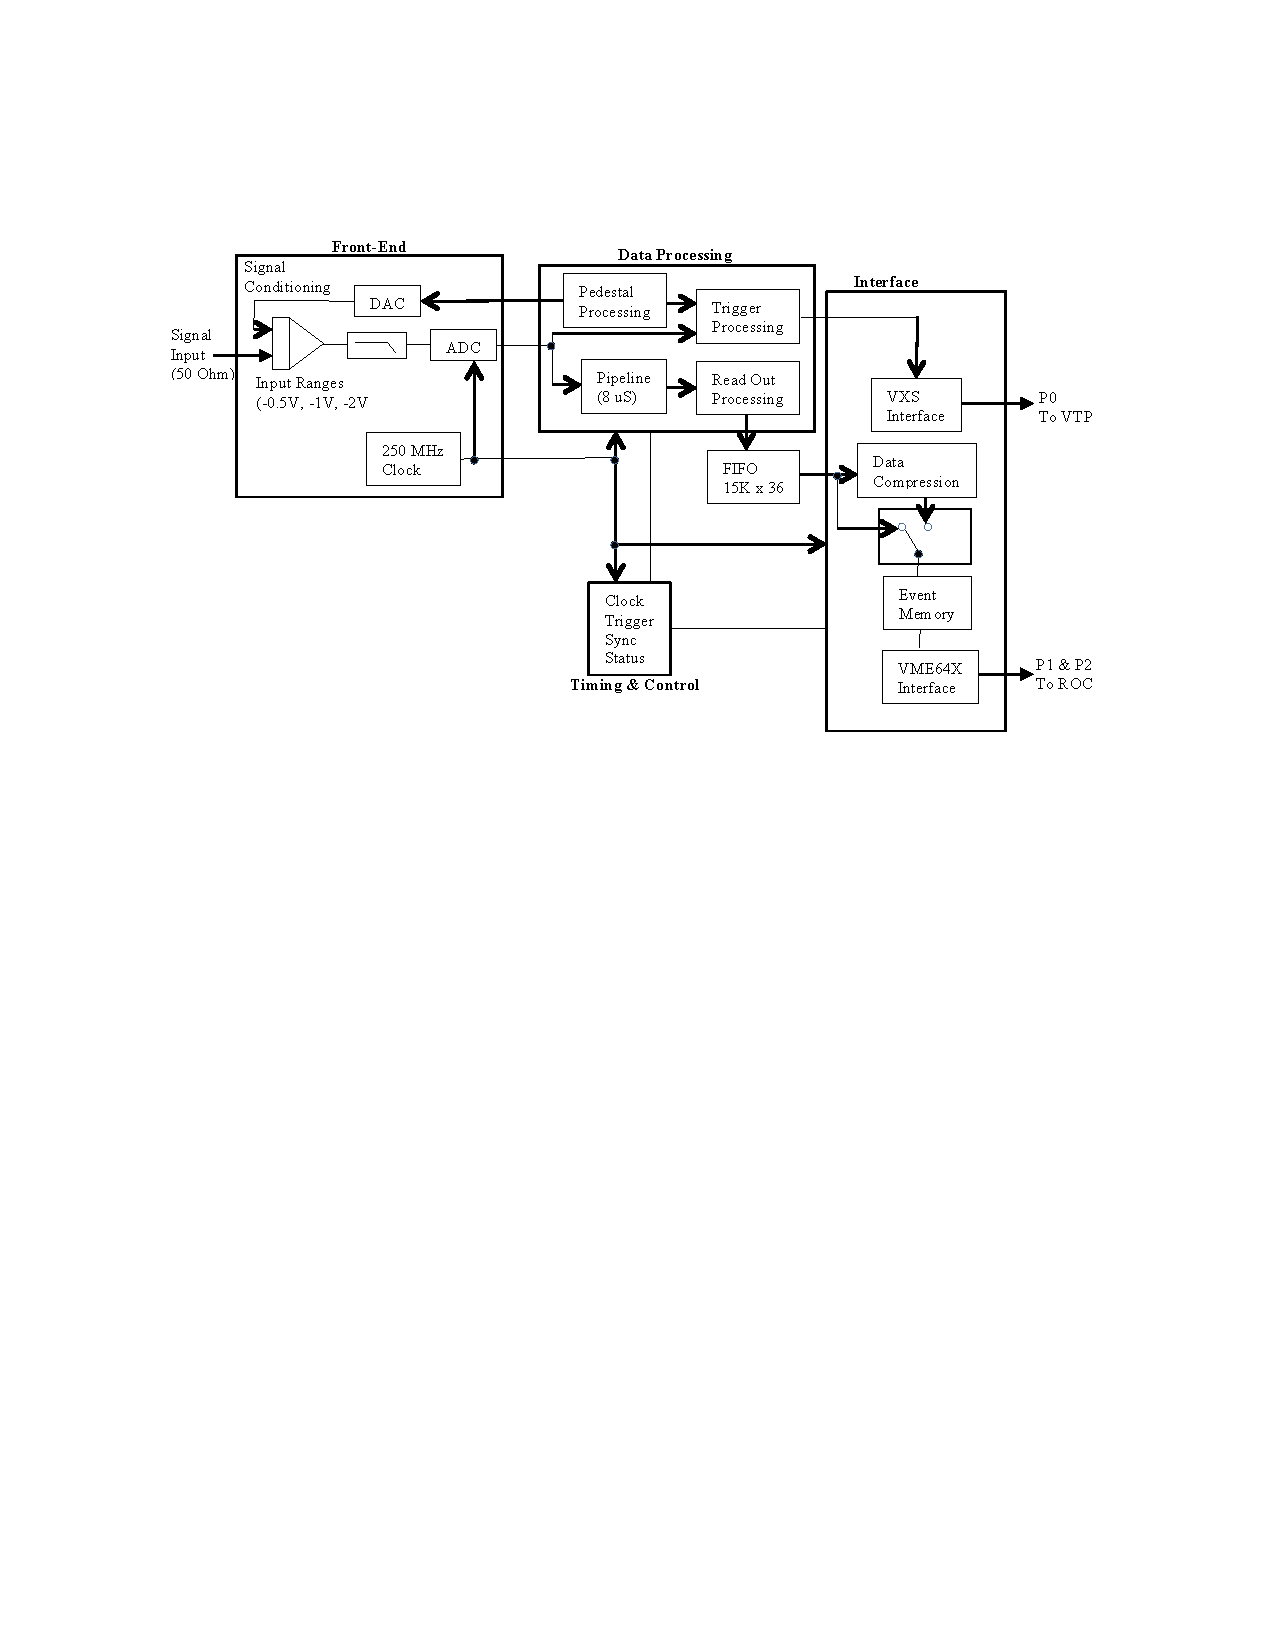
\includegraphics[width=1.0\columnwidth,keepaspectratio]{img/FADC250_Diagram.pdf}
	\caption{Flash ADC module diagram (FADC250)}
	\label{fig:FADC250_board}
\end{figure}

Digitized data from the 16 FADC chips is processed and formatted for readout in a pair of high performance Xilinx FPGAs. The digitized data from the ADCs follows two distinct paths.  Logic in the trigger data path pre-processes data for the trigger algorithms of the VXS Trigger Processor (VTP). The FADC250 module continuously streams this data to the crate VTP located in VXS switch slot A via high-speed serial links of the VXS fabric.  Data from multiple VTPs and other modules are used to form a global trigger signal that is returned to the crates to initiate data readout.

The readout data path continuously stores digitized data for each channel in circular buffers. When a trigger signal is received by the module a programmable window up to 2 $\mu$s wide of digitized data is extracted from the buffers for processing. The starting point of this window can be programmed up to 8 $\mu$s earlier than the arrival of the trigger signal to account for the time required to form the trigger signal.  Zero suppression on the extracted data may be implemented for each channel using programmable thresholds.  A lossless data compression algorithm can also be applied to the data of each channel with typical compression factors of 2 to 3. The design is pipelined so that data from multiple triggers can be processed simultaneously.  Triggers separated in time by as little as 50 ns can be accepted by the module. The trigger number and trigger time (clock periods since last synchronization) are reported along with the channel data so that data from multiple modules can be correctly assembled into events. 

Data associated with a programmable number ``N'' of triggers is packaged into a block of data for read out over VME.  ``N'' can take values from 1 to 255, with 40 being a typical value chosen.  Data is stored in an on-board 8 MB SRAM as 64-bit words to match the 64-bit high-speed (200 MB/s) dual edge VME Source Synchronous Transfer (2eSST) mode employed to read out the module.  

In order to save the overhead of setting up a DMA transfer for each FADC250 module in the crate, a chained block readout mechanism with token passing is used.  A common address range is enabled for all modules in the crate but only the module having the token will respond to a read request.  A single logical DMA read is initiated by the VME crate controller and the first module in the chain supplies data from its block of event fragments.  When the block data from the first module is exhausted, a token signal is passed to the next module in the chain and this module then proceeds to transmit its data from its block.  When the block for the data from that module is exhausted, it transfers the token to the next module.  This continues until the data from the last module in the chain is exhausted.  Instead of passing the token the last module asserts the VME bus error signal (BERR), which terminates the DMA cycle.  The user returns the token to the first module and the process can begin again when the next block of events is ready for readout.  The user does not have to query the modules in advance to discover the number of words to read out.  The DMA is set up with a total number of words larger than any expected value for the entire crate.  Data from each module is tagged with the slot number to identify its source.  The token passes along a VXS signal line to VXS switch slot B, where a module there (SD) routes it to the next enabled module.


\subsection{Discriminator Scaler Module (DSC2)}

The Discriminator Scaler Module (DSC2 \cite{dsc2-ref}, see Fig.~\ref{fig:dsc2_board}) is a 16-channel general purpose discriminator and scaler module designed as a 6U VME card. It replaces an older design, improving on jitter, noise, crosstalk, and adding new features.

\begin{figure}[hbt]
	\centering
	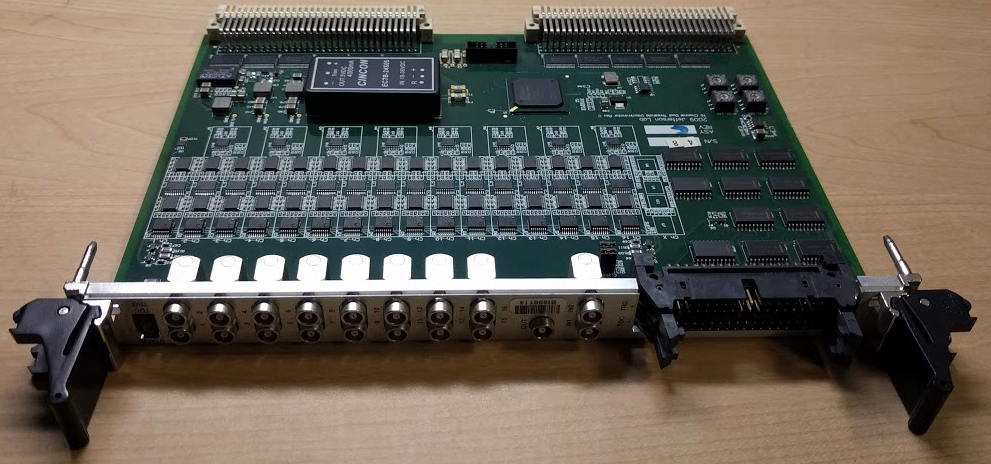
\includegraphics[width=1.0\columnwidth,keepaspectratio]{img/dsc2_board.png}
	\caption{Discriminator Scaler module (DSC2)}
	\label{fig:dsc2_board}
\end{figure}

\begin{center}
	DSC2 Specifications\\
	\begin{tabular}{| l | l |}
		\hline \hline
		Property			& Value				\\
		\hline
		{\bf Analog Discriminator}	&				\\
		Threshold			& 0 to -1023 mV			\\
		Pulse width			& 4 ns to 40 ns			\\
		Dead-time			& 4 ns typ. w/8 ns pulser width	\\
		Maximum input rate		& $>$125 MHz 			\\
		Ch-ch isolation			& $>$65 dB			\\
		Threshold noise			& 1.3 mV RMS (typical)		\\
		Slew-rate delay disperson	& $<$20 ps			\\
		Input-to-output delay		& $<$5 ns			\\
		{\bf Digital Processing}	&				\\
		Digital delay step		& 4 ns				\\
		Digital delay maximum		& 1 us				\\
		Digital width maximum		& 1 us				\\
		Maximum count rate		& 125 MHz			\\
		\hline \hline
	\end{tabular}
\end{center}

\paragraph{Discriminator}
Inputs are single-ended LEMO and leading-edge discrimated by two different thresholds. Typically one threshold is used for time-to-digital applications and the other threshold is used for trigger applications. There are separate differential ECL outputs for each channel and threshold. Low jitter performance was an important goal of the design as this module will be used in high resolution applications. Fig.~\ref{fig:dsc2_jitter} shows the typical jitter as a function of a variety of input slew rate signals and threshold overdrive conditions.

\begin{figure}[hbt]
	\centering
	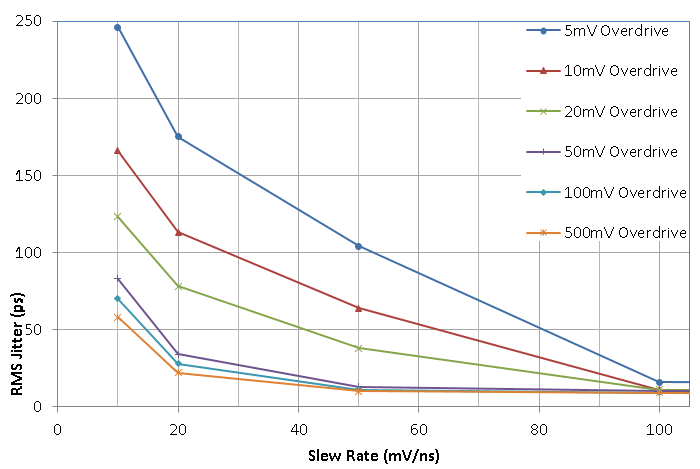
\includegraphics[width=1.0\columnwidth,keepaspectratio]{img/dsc2_jitter.png}
	\caption{Output Jitter vs Input slew rate and overdrive}
	\label{fig:dsc2_jitter}
\end{figure}

\paragraph{Digital Processing}
A Xilinx Spartan 3A FPGA is used to implement the VME interface, scalers, discriminator controls, and scaler event building features. Each channel and threshold has two scalers associated with it. The first scaler counts all threshold crossings for the input. The second scaler is gated using a front-panel input source, which can be useful to computing dead-time of channels and many other applications. Additionally, reference scalers are accumulated (a gated and ungated version) that count the elapsed time, which can be used to normalize inputs scalers to Hz. All together there are 68 scalers, which can be slow to read over VME if using single-cycle transfers. An event builder is implemented that can synchronously read (and optionally clear) all scalers and build an event with this data. Over 100 events can be buffered and readout using the VME 2eSST protocol at 200~MB/s.


\subsection{TDC Modiles (v1190/v1290)}

Commercial CAEN V1190/V1290/V1290N TDC \cite{tdc-ref} boards are used for timing measurements in the PMT-based CLAS12 detectors (see Fig.~\ref{fig:v1190_board}). The V1190 has timing resolution about 100~ps and the V1290 about 35~ps. All boards installed in CLAS12 run on an external 250/6=41.666~MHz clock rather then internal 40~MHz clock. The use of a different clock required compensation table remeasuring and reloading.

\begin{figure}[hbt]
	\centering
	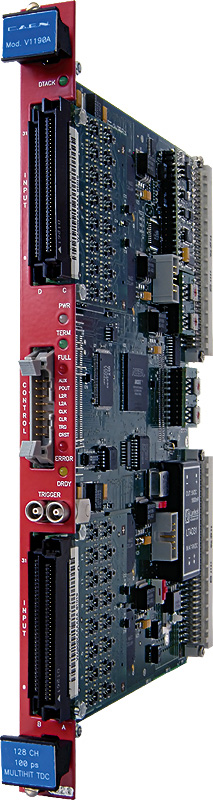
\includegraphics[width=0.2\columnwidth,keepaspectratio]{img/v1190_board.jpg}
	\caption{CAEN V1190 TDC module (V1190)}
	\label{fig:v1190_board}
\end{figure}

\subsection{Drift Chamber Readout Board (DCRB)}

\begin{figure}[hbt]
	\centering
	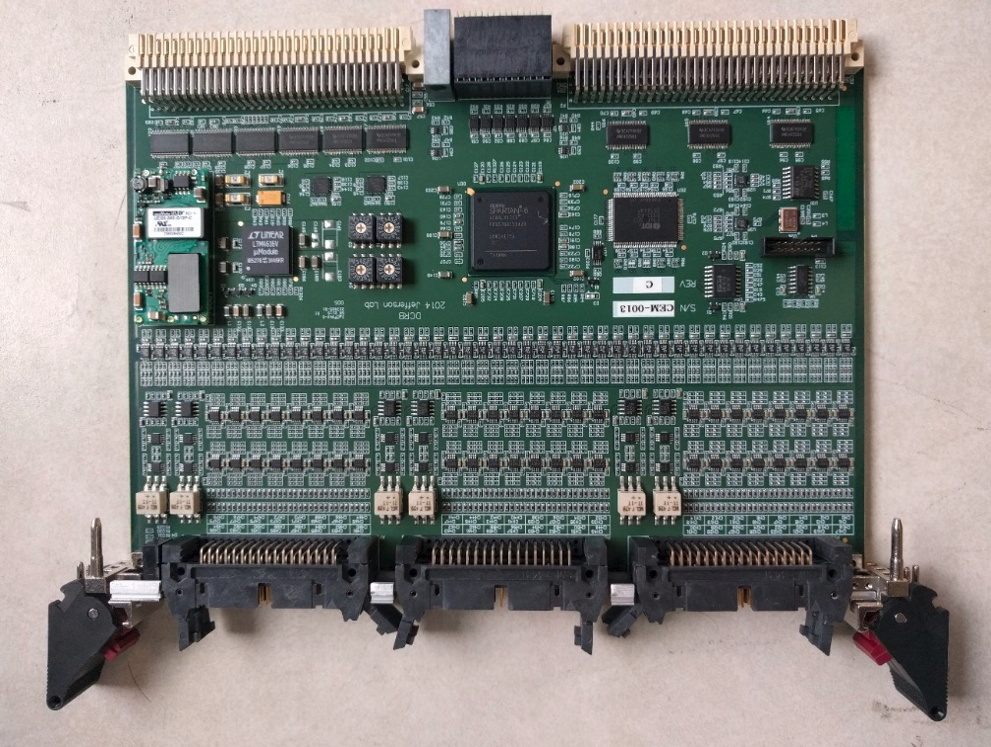
\includegraphics[width=1.0\columnwidth,keepaspectratio]{img/dcrb_board.png}
	\caption{Drift Chamber Readout Board (DCRB)}
	\label{fig:dcrb_board}
\end{figure}

The Drift Chamber Readout Board (DCRB \cite{dcrb-ref}, see Fig.~\ref{fig:dcrb_board}) is a 96-channel amplifier, discriminator, and time-to-digital converter module used to digitize and readout hits from the CLAS12 Drift Chambers. A single VXS crate of DCRB modules can readout a full region of the drift chambers for a single sector resulting in 18 VXS crates of DCRBs to instrument 6 sectors each having 3 regions of drift chamber.

\paragraph{Analog Inputs}
Each DCRB receives 96 differential analog signal pairs using twisted pair cabling from the drift chamber pre-amplifiers. The pre-amplfiers located on the detector provide a gain of ~2.3~mV/$\mu$A. On the DCRB each analog input channel is amplified by a voltage gain of 30 and then discriminated by a programmable threshold (common to all channels on the board with an effective chamber wire threshold range of 0 to 3.5/$\mu$A).

\paragraph{TDC Event Builder}
All discriminated channels go to a Xilinx Spartan 6 FPGA where a 96-channel 1~ns resolution time-to-digital converter (TDC) is implemented in firmware. The TDC is based on the ISERDES2 shift register FPGA primitive that directly samples of the digital input with a single-data-rate (SDR) input register clocked at 1~GHz. The TDC sampling clock is synchronized to the CLAS12 master oscillator, making it easy to relate hit times in the drift chamber to the other detectors in CLAS12. The TDC inputs are buffered to support multiple hits, allowing for an average hit rate of 4~MHz per input before loss of data, which exceeds the chamber design hits rates by a few orders of magnitude. Hits from groups of 16 channels are written into a large buffer that a linked-list content addressable memory (CAM) tracks for 16~$\mu$s. When a L1A trigger signal is received, a time window of hits is extracted from the TDC hit buffer. The readout window times are supplied to the CAM, and the CAM provides the address of the last hit matching each readout time bin. The hit buffer is then read to extract the hit and also the address of the next hit in the buffer matching the time bin (this is the linked list behavior). The result is an extremely fast event builder with natural zero suppression that does not require time sorted data. Cleanup is accomplished by a timer that invalidates the CAM entries after time bins are older then 16~$\mu$s. Hits for an event are assembled and buffered in a 2~MByte external RAM, which is readout through the VME bus using the 2eSST protocol at 200~MB/s.

\paragraph{Calibration Support}
A programmable amplitude pulse generator is implemented that can inject test pulses directly into the DCRB differential amplifier inputs as well as to the pre-amplfiers that are on the detector. This provides a way to test points of failure, check channel gain, and check channel delays without any extra equipment. A scaler is implemented on each channel for slow control monitoring of all chamber wires.

\subsection{VXS Silicon Readout Module (VSCM)}
The CLAS12 Silicon Vertex Tracker detector (SVT, \cite{svt-ref}) front-end utilizes the data driven FSSR2 ASIC for digitization. The VXS Silicon Readout Module (VSCM \cite{vscm-ref}, Fig.~\ref{fig:vscm_board}) was designed to interface the FSSR2-based front-end to the CLAS12 DAQ system. This system is capable of reading out all 33,792 SVT channels in 3 VXS crates.

\begin{figure}[hbt]
	\centering
	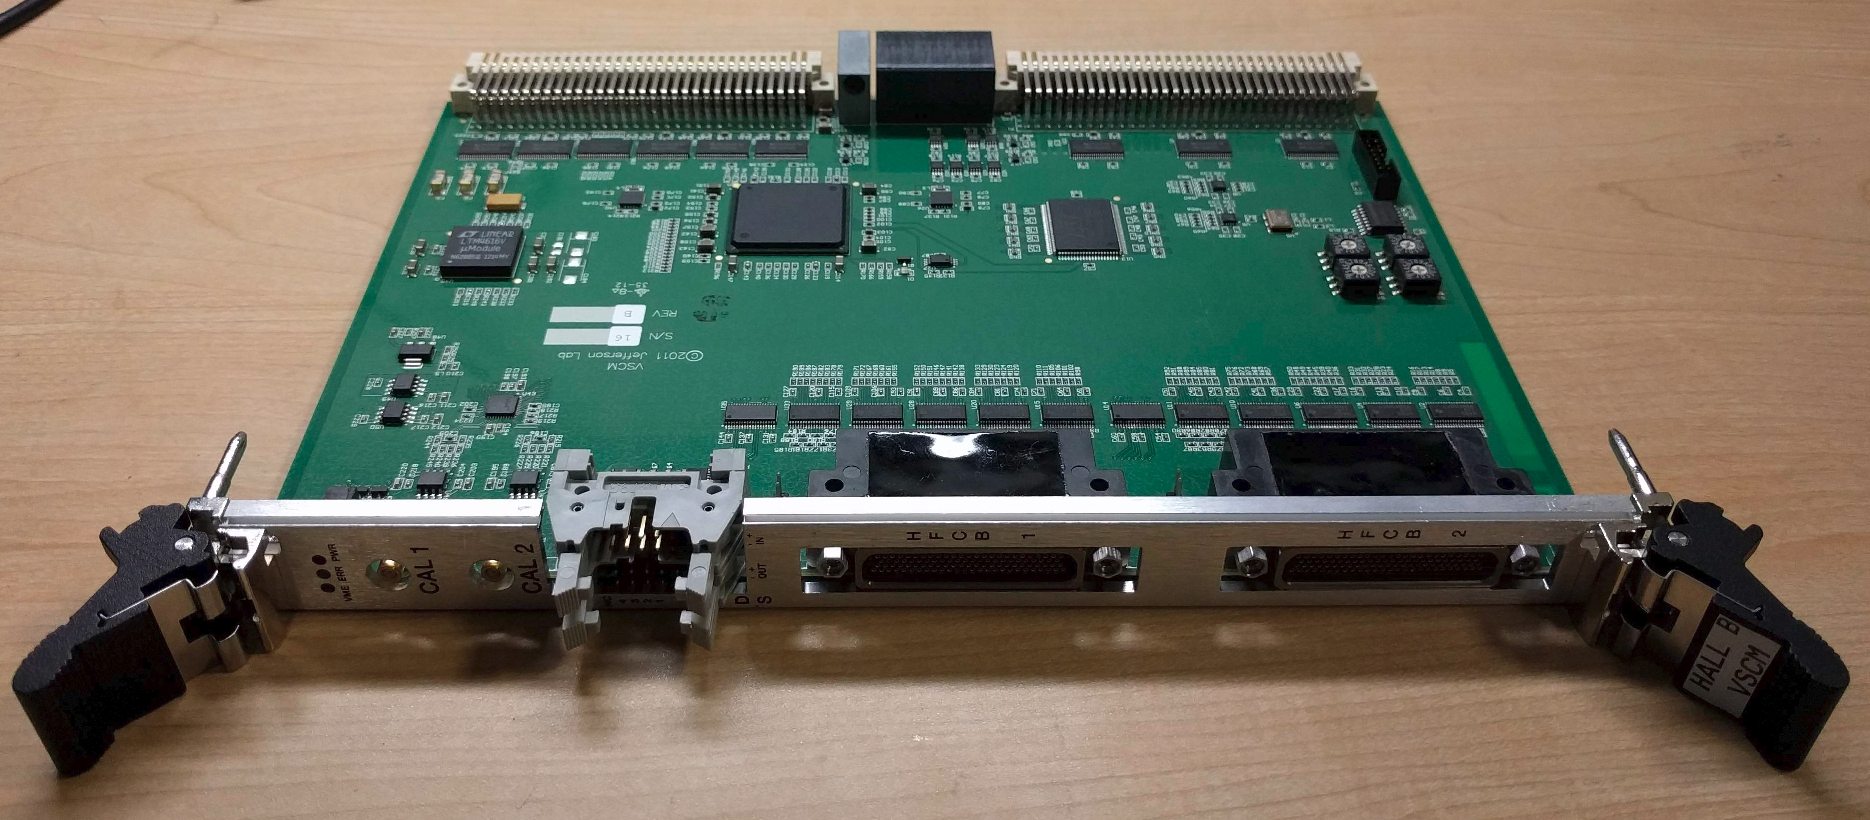
\includegraphics[width=1.0\columnwidth,keepaspectratio]{img/vscm_board.png}
	\caption{VXS Silicon Readout Module (VSCM)}
	\label{fig:vscm_board}
\end{figure}

The main features of the VSCM include:

\begin{itemize}
	\item Receives 8 FSSR2 streams, each at 840~Mbps
	\item De-randomizes hits into an 8~$\mu$s buffer
	\item 512k hit, multi-event buffer
	\item Supports $>$1~MHz trigger rate
	\item Programmable amplitude charge injector
	\item 1~ns resolution time-to-digital converter (TDC)
	\item Per channel hit scaler
	\item FSSR2 synchronization, status, and control
\end{itemize}

\paragraph{Event Builder}
The VSCM deserializes the FSSR2 streams, checks for errors, and decodes the hits, which are stored in an 8~$\mu$s circular memory. The hits are not guaranteed to be time ordered, so the timestamp and channel number are used to form the circular memory address (rather than storing in the order received). The VSCM also implements an 8-channel 1~ns time-to-digital converter (TDC) that measures the logic OR of hits from each FSSR2 ASIC. This high time resolution is significantly better than the FSSR2 serial stream hit time resolution and is required for improved out-of-time hit rejection. The L1A trigger signal time is used to look back a fixed amount of time and extract a time window of hits from the circular memory, which corresponds to the physics event. Non-zero hits are assembled as an event and buffered in a 2~MByte external RAM that is readout through the VME bus using the 2eSST protocol at 200~MB/s.

The event data contains primarily two hit word types that together provide high time resolution and spatial hit resolution while keeping the front-end complexity low.

\begin{center}
	Low time resolution hit word\\
	\begin{tabular}{| l | l |}
		\hline \hline
		Property	& Description		\\
		\hline
		Hit Time	& 128~ns resolution	\\
		Channel		& 0-1023 strip ID	\\
		Charge		& 0-7 threshold		\\
		\hline \hline
	\end{tabular}
\end{center}

\begin{center}
	High time resolution hit word\\
	\begin{tabular}{| l | l |}
		\hline \hline
		Property	& Description		\\
		\hline
		Hit Time	& 1~ns resolution	\\
		Channel		& 0-7 chip ID		\\
		\hline \hline
	\end{tabular}
\end{center}

Fig.~\ref{fig:vscm_blockdiagram} shows the hardware block diagram of the module. Essentially, a single low-cost Xilinx Spartan 6 FPGA was used to implement the deserialization, buffering, event-building, monitoring, front-end configuration, time-to-digital conversion, and monitoring.

\begin{figure}[hbt]
	\centering
	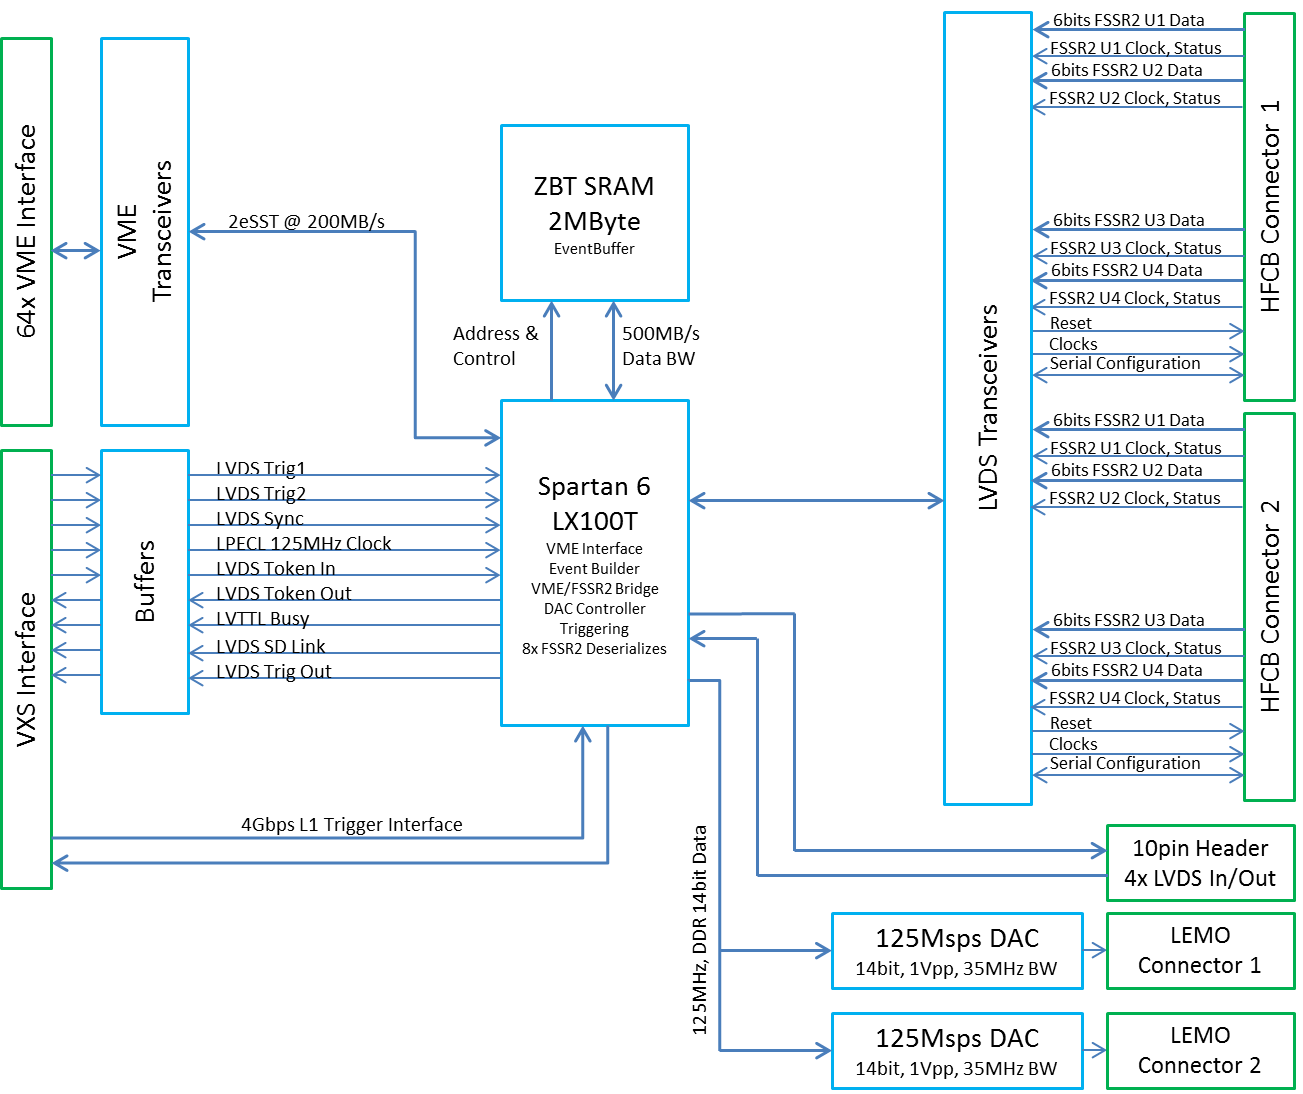
\includegraphics[width=1.0\columnwidth,keepaspectratio]{img/vscm_blockdiagram.png}
	\caption{VSCM Hardware Diagram}
	\label{fig:vscm_blockdiagram}
\end{figure}


\subsection{SSP Board as ffber Readout Module}

The SubSystem Processor (SSP \cite{ssp-ref}) was originally designed to work as part of CLAS12 Trigger System. It is used to readout some front-end electronics in the DAQ system as well. The board description can be found in the CLAS12 Trigger System article \cite{trig-ref}.
\section{Software}

\subsection{... CODA DAQ software ... (Abbott)}

CLAS12 DAQ system is based on CODA (Fig.~\ref{fig:coda_diagram}), short for CEBAF Online Data Acquisition. It is a kit of parts that allows the researcher to implement a data acquisition system. The scale of the system can range from a few detector channels in a test stand to tens of thousands of channels in a large detector installation in one of the halls. CODA achieves this scaling through modularity and provides a set of hardware components along with complementary software components.

\begin{figure}[hbt]
	\centering
	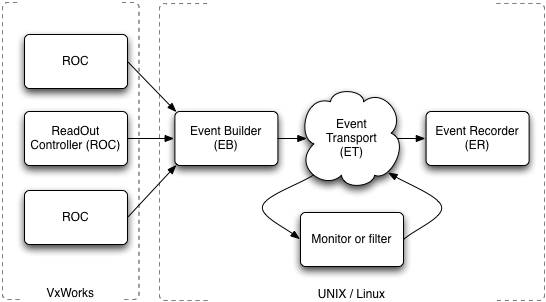
\includegraphics[width=1.0\columnwidth,keepaspectratio]{img/coda_diagram.png}
	\caption{CODA System Diagram}
	\label{fig:coda_diagram}
\end{figure}


\subsection {Runcontrol(Sergey)}

The CODA DAQ system includes a run control facility consisting of a back-end run control supervisor and a front-end graphical operator display that connects to the supervisor and controls its operation. The supervisor in turn controls operation of the many CODA components that participate in the run. The latter are defined in run configuration files that the operator chooses at startup. The gui presents the operator with a choice of possible actions that depend on the current state of the run. The supervisor translates the operator choice into appropriate commands to the individual components. Alternatively, limited communication with the supervisor can be performed via command-line scripts.
The supervisor in addition monitors the health and operation of the CODA components and warns the operator or pauses the run if problems are detected.


\subsection{Front End Libraries(Moffit)}

\subsection{Frontend Libraries}

Just an outline ATM

GEFANUC driver:
\begin{itemize}
\item Customized Kernel Driver and Userspace Interface
\item C API provides:
   \begin{itemize}
   \item Setup of VME inbound and outbound windows
      \begin{itemize}
      \item Permanent windows: CRCSR, A16, A24, A32
      \item Map of these windows into userspace
      \end{itemize}
   \item Allocate of Physical Memory for DMA
      \begin{itemize}
      \item Map of this memory into userspace
      \end{itemize}
   \end{itemize}
\end{itemize}

JVME Userspace Driver:
\begin{itemize}
\item C API provides
  \begin{itemize}
  \item common userspace interface to GEFANUC driver and others.
  \item Initialization of kernel driver and default VME windows
  \item Maps VME bridge registers into userspace
    \begin{itemize}
    \item Provides userspace configuration and operation of DMA
    \end{itemize}
  \item Initialization of and access to shared memory mutex for intra-process cooperation during DMA
  \end{itemize}
\end{itemize}

Frontend Libraries
\begin{itemize}
\item C APIs provide
  \begin{itemize}
  \item module register mapping in VME windows to memory structures.
  \item configures modules for readout via
    \begin{itemize}
    \item programmed i/o
    \item Single module DMA
    \item Multiple module DMA
       \begin{itemize}
       \item Token passing (P0/VXS and CBLT) with common A32 address range
       \item Linked List DMA
       \end{itemize}
    \end{itemize}
  \end{itemize}
\end{itemize}



\subsection{Readout Controller(Abbott)}

Readout Controller (ROC, Fig.~\ref{fig:roc_diagram}) software component is the program running on front-end controllers such as Intel-based VME/VXS crate controllers, VTP trigger boards or regular Linux servers - any hardware receiving data from front-end electronics. On the DAQ startup ROC main program starts three threads, after that it just controlls thread health and communicates with run control process. Three threads (readout, processing and network) are passing data from one to another communicating over circular buffers. Typical number of buffers in each circle is 8 and size of every buffer is 4 MBytes, which defines how long front-end electronics will be read out before feeling effect of the back-end busy conditions.

First (readout) thread receives data from front-end electronics and places them into first circular buffer. That thread can run in pooling mode occupying entire cpu core, or in interrupt mode. CLAS12 are using mostly pooling mode which has adequate performance on multi-core controllers.

Second (processing) thread reads data from first circular buffer and perform needed data processing, in particular it does so-called disentangling and data sanity check. Results placed into second circular buffer. That component can create its own threads to burst processing power.

Third (network) thread reads data from second circular buffer and send it over network to the Event Builder.

First and second threads have user part which compiled separately and downloaded dynamically, it allows users to develop experiment-dependent code without recompiling CODA framework.

\begin{figure}[hbt]
	\centering
	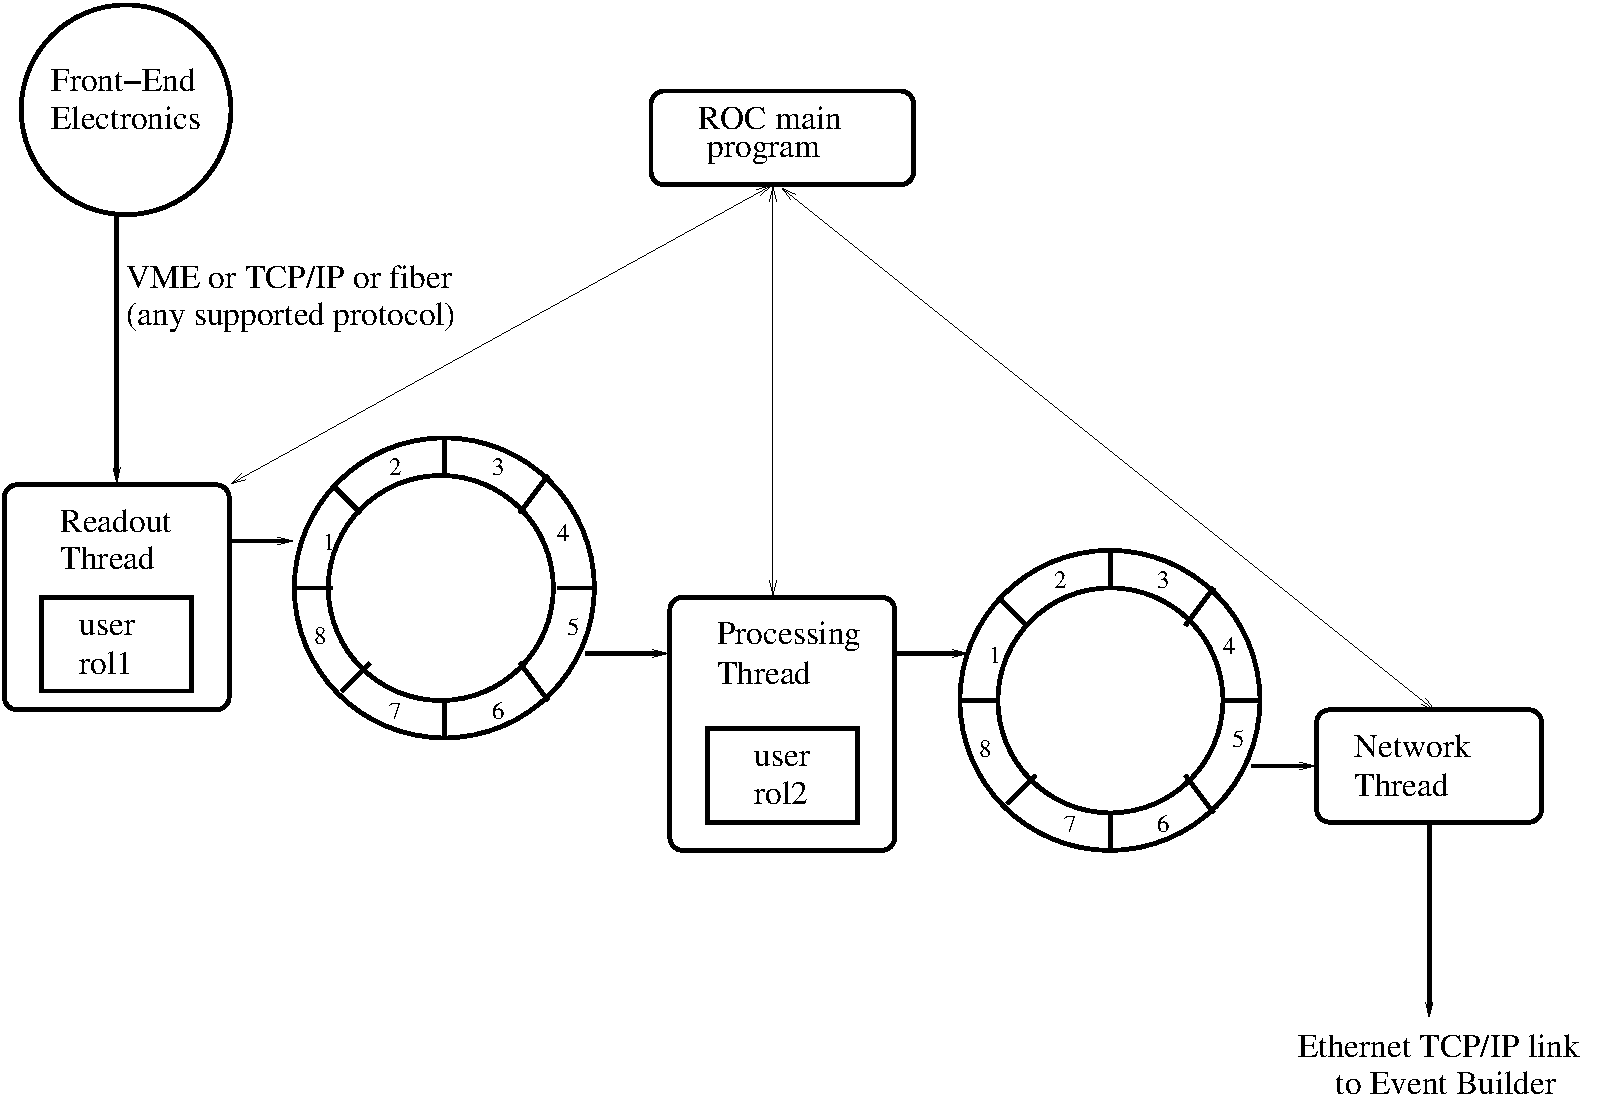
\includegraphics[width=1.0\columnwidth,keepaspectratio]{img/roc_diagram.pdf}
	\caption{Readout Controller Diagram}
	\label{fig:roc_diagram}
\end{figure}


\subsection{Event Builder (Graham)}

Event Builder (EB, Fig.~\ref{fig:eb_diagram}) is the program receiving data fragments from all readout controllers and glueing it into events. Building process is based on event number, event type and timestamp of the data fragments: for every particular event all three values have to be identical for all data from all readout controllers. In case of any difference DAQ will be stopped and error reported.

Event Builder consists of receiving and building parts. Receiving part contains set of independent threads, one per readout controller connected to it by TCP protocol. Every thread receives data and place it into internal buffer. If buffer becomes full thread stops receiving data, effectively propagating busy condition back to readout controller.
Building part has the number of identical building threads, which takes turns by getting data from receiving part internal buffers, building events and placing them into Event Transfer System.

Total number of Event Builder threads in CLAS12 DAQ is currently 118, so the number of network connections from readout controllers. Because of that it have to run on powerful server, usually the one with many cpu cores, big memory and high bandwidth network card. CLAS12 is using DELL R730 server with 32 cores, 64GByte memory and 40Gbit network card. That server is adequate for CLAS12 DAQ requirements.

\begin{figure}[hbt]
	\centering
	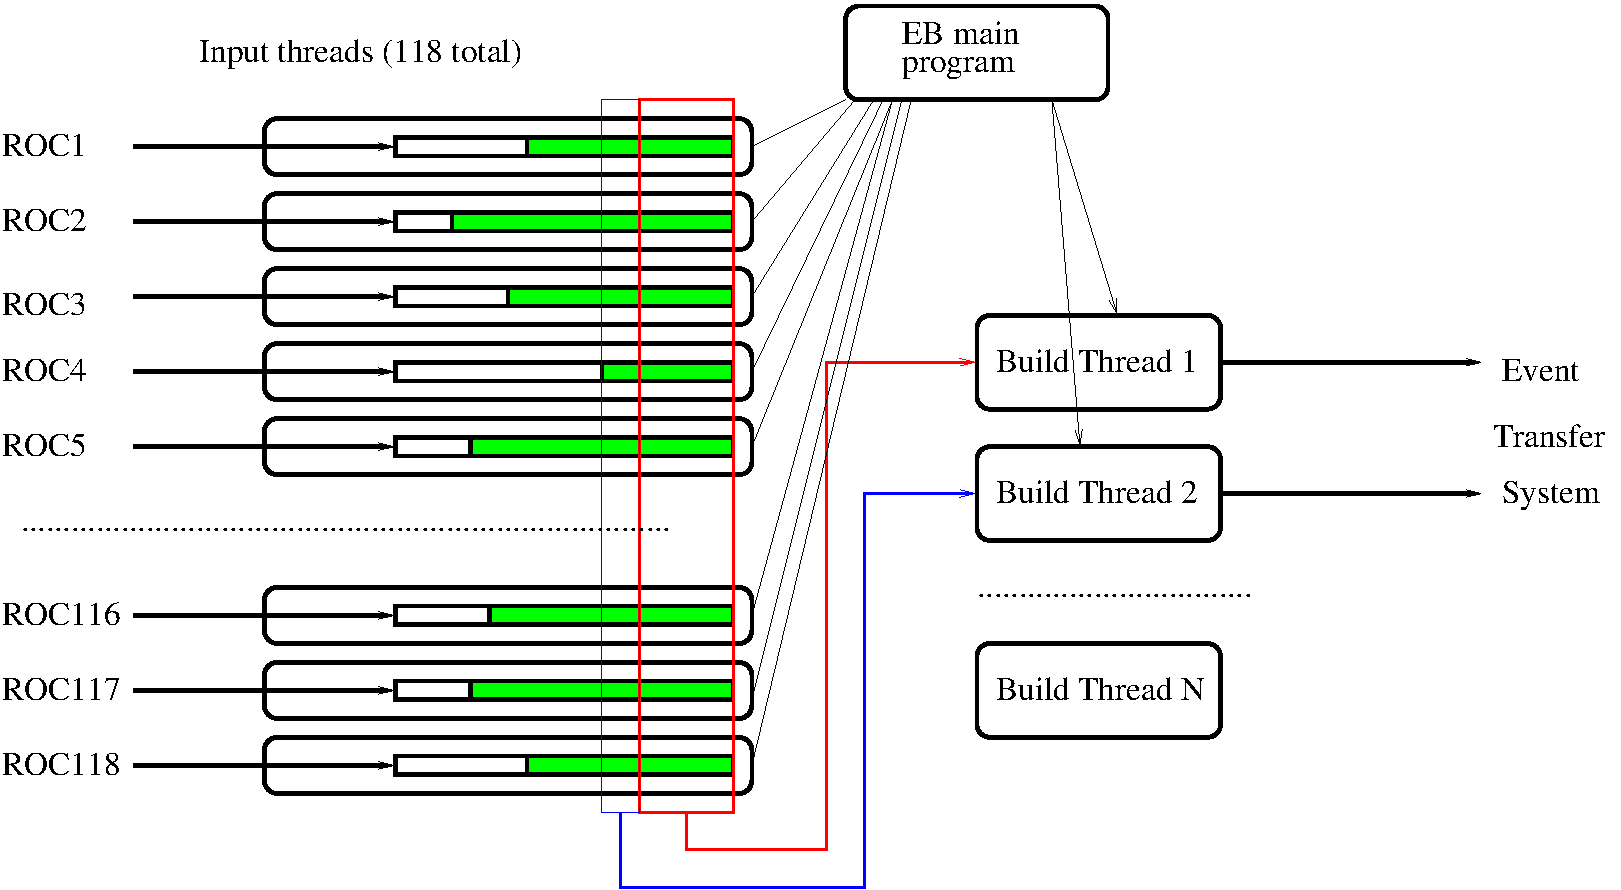
\includegraphics[width=1.0\columnwidth,keepaspectratio]{img/eb_diagram.pdf}
	\caption{Event Builder Diagram}
	\label{fig:eb_diagram}
\end{figure}


\subsection{Event Transfer (Carl)}

Event Transfer (ET) system allows multiple connections to the data stream, needed for online data monitoring and possibly data or/and event reduction. It consists of ring of buffers, one per event, filled by Event Builder and accessed by one or several processing programs. Every processing program can request to see every event or subset of events based on selecting algorithm. There is a possibility to access ET system remotely, as well as create a chain of ET systems running on different servers effectively increasing processing power. Last program attached to ET system usually Event Recorder.

\subsection{Event Recorder (Sergey)}

Event Recorder (ER) is the program receiving data from ET system and recording data files into the disk. It can write data in one or several files in parallel (so-called multi-stream mode). If multi-stream mode is used event order is preserved, but it requires the allocated memory size to be bigger then the number of streams multiplied by the file size.


\subsection{Messaging System (ActiveMQ) (Sergey)}

Messaging system in CLAS12 DAQ is based on ActiveMQ library and its C++ extension. Two ActiveMQ servers used to route all communiations. The number of connections to ActiveMQ is several hundreds, and the number of messages sent every second is several tens of thousands, with data volume few tens of Megabytes per second. Messaging system is used in particular to monitor and control DAQ components, in addition to the Runcontrol.


\subsection{Runtime Database (RCDB) (Sergey)}

JLAB-designed mysql-based Runtime Database (RCDB) is used to store run parameters and statistic. It has web interface (Fig.) and provides interface to various languages including C++ and Java.


\subsection{Online Data Monitoring (Raffaella,Cole)}

CLAS12 Online data monitoring is the set of programs attached to Event Transfer System and processing data in real time. One of such program's output is shown on Fig.



\subsection{CSS for DAQ, communication with DAQ (Nathan)}



\subsection{ROOT for DAQ (FT) (Andrea)}

A ROOT-based system was developed to display integrated quantities from the CLAS Trigger system in the form of 1D
and 2D histograms. The system is made by three different applications: a histogram sender running on each VTP, a
histogram receiver running on a DAQ server, and a user-configurable GUI client. Each histogram sender application
defines a set of 1D and 2D histograms to report trigger data specific to the CLAS12 subsystem handled by the VTP it is
running on. Histograms are refreshed at a fixed rate and streamed to the DAQ server in the form of JavaScript Object
Notation (JSON) messages, exploiting the previously described ActiveMQ infrastructure. Each message contains: the
histogram name, the number of bins, and a data array with the number of counts in each bin. The message receiver
application is responsible for decoding these messages, and of creating ROOT histograms from them. Finally, the client
application displays ROOT histograms to the user through a customizable GUI.

The GUI is composed of a programmable number of independent frames, with different histograms in each of them.
Typically, each frame contains histograms related to the same CLAS12 subsystem. The GUI structure is specified through
a configuration file passed as a command-line option when running the client. Communication between the message
receiver/ROOT histogram produced application and the user client is handled through the ROOT TSocket mechanism.
Figure~\ref{fig:plot_andrea} shows a GUI reporting histograms from the Forward Tagger system~\cite{ft-ref}: two
2D histograms showing the distribution of electromagnetic cluster hits in the Forward Tagger Calorimeter, and two
1D histograms showing the electromagnetic cluster energy distribution. The right (left) column reports histograms for
electromagnetic clusters  with (without) a matching hit in the Forward Tagger Hodoscope.

\begin{figure}[t]
	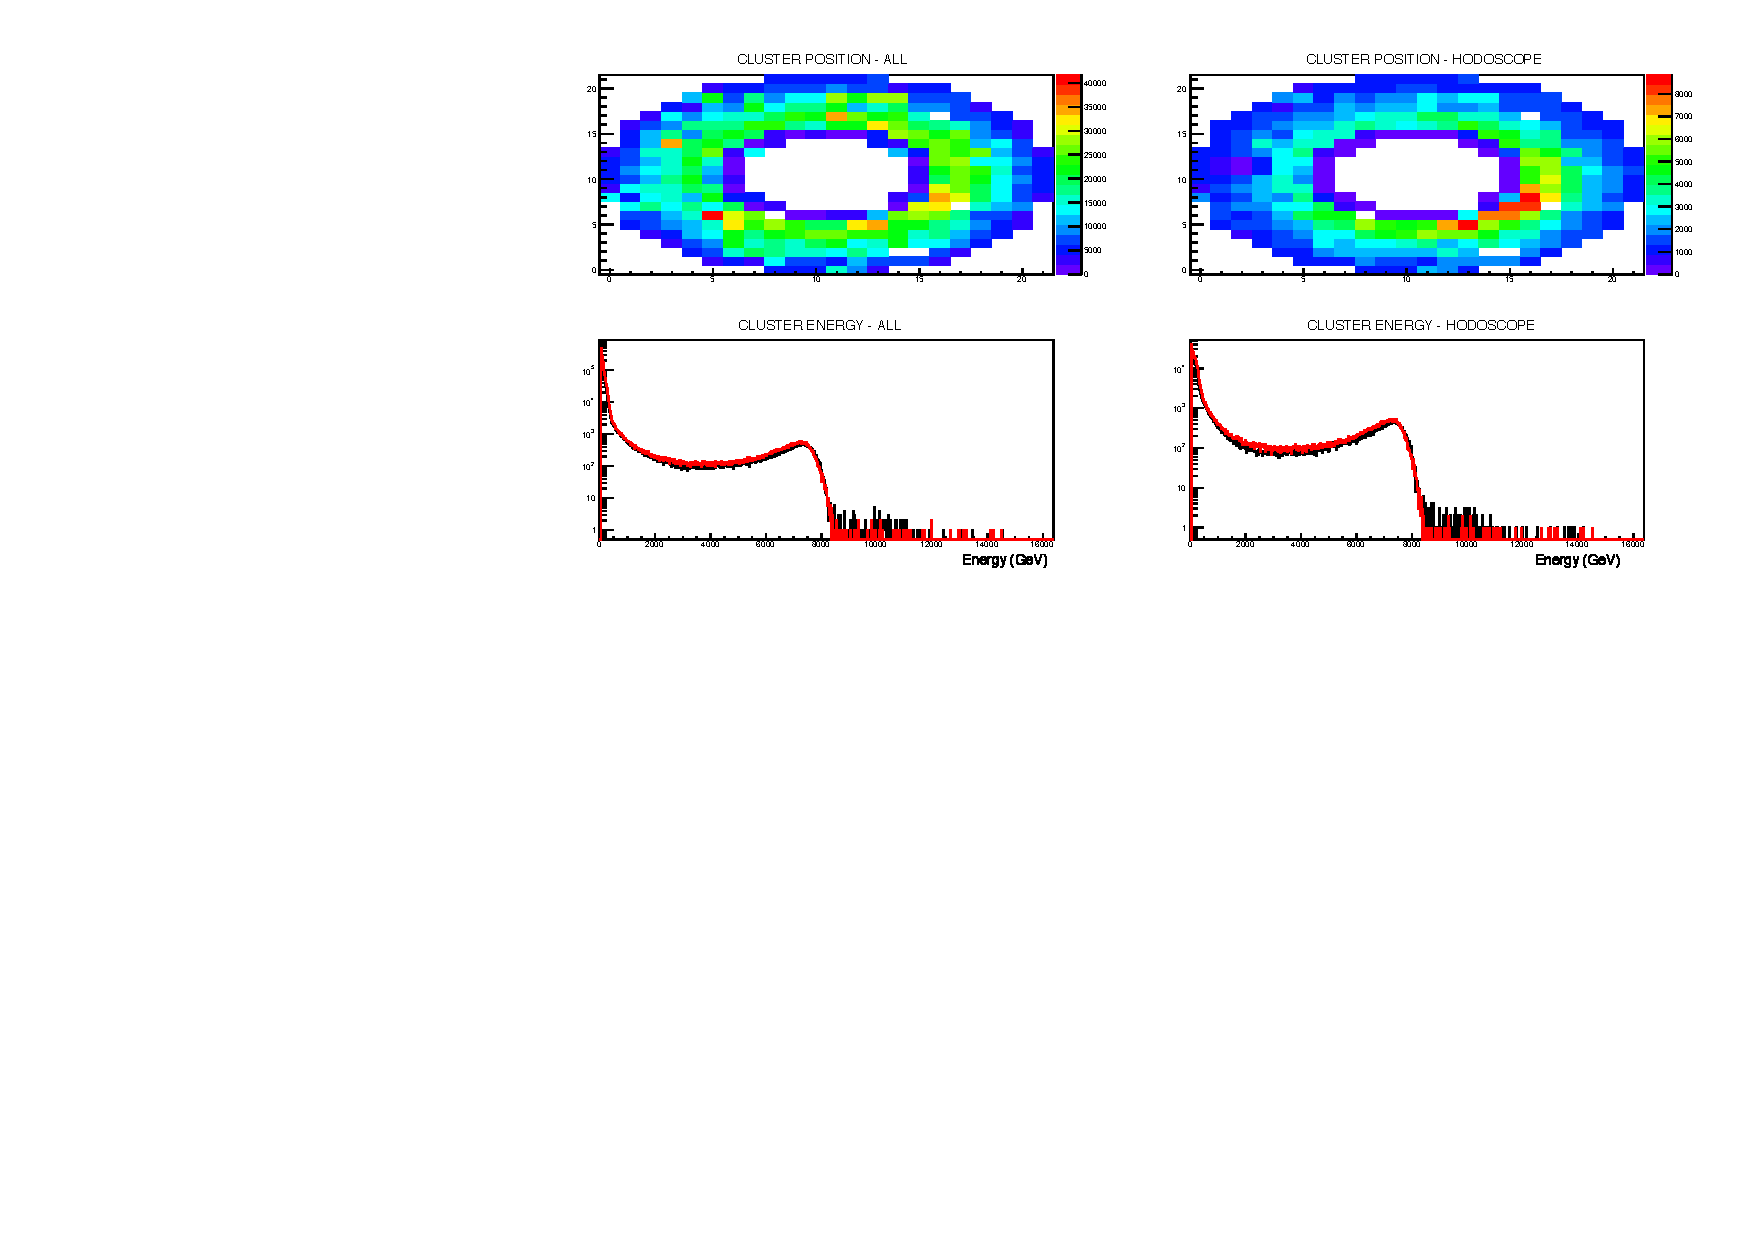
\includegraphics[width=1.0\columnwidth]{img/plotAndrea.pdf}
	\caption{Example of a ROOT-based GUI to monitor trigger data for the specific case of the Forward Tagger
        detector~\cite{ft-ref}. The top histograms report the distribution of electromagnetic cluster hit positions, while
        the bottom histograms report the electromagnetic cluster energy distribution. The right (left) column reports
        histograms for electromagnetic clusters  with (without) a matching hit in the Forward Tagger Hodoscope.}
	\label{fig:plot_andrea}
\end{figure}



\subsection{CLAS Event Display (Heddle)}

The CLAS12 event display (ced) is a full-function graphical application that displays on-line (and off-line) events using various representations of CLAS12 called views. The views are independent windows that the user can pan, zoom, scroll, etc. Some of the views are geometrically faithful, and some are designed for maximal information content as opposed to realism. The primary purpose and utility of ced, when used on-line as part of the DAQ system, is for additional monitoring. While running, ced will display an event from the live stream at a selectable rate, typically one every two seconds. A quick glance at ced will confirm, for example, that there are data in the drift chambers that appear to form tracks. In this way it serves as an early warning of problems with detectors and/or the data stream. It is also possible to operate ced in a mode where it creates graphical histograms or occupancy overlays. A typical view from ced is shown in Fig.~\ref{fig:ced}.

\begin{figure}[hbt]
	\centering
	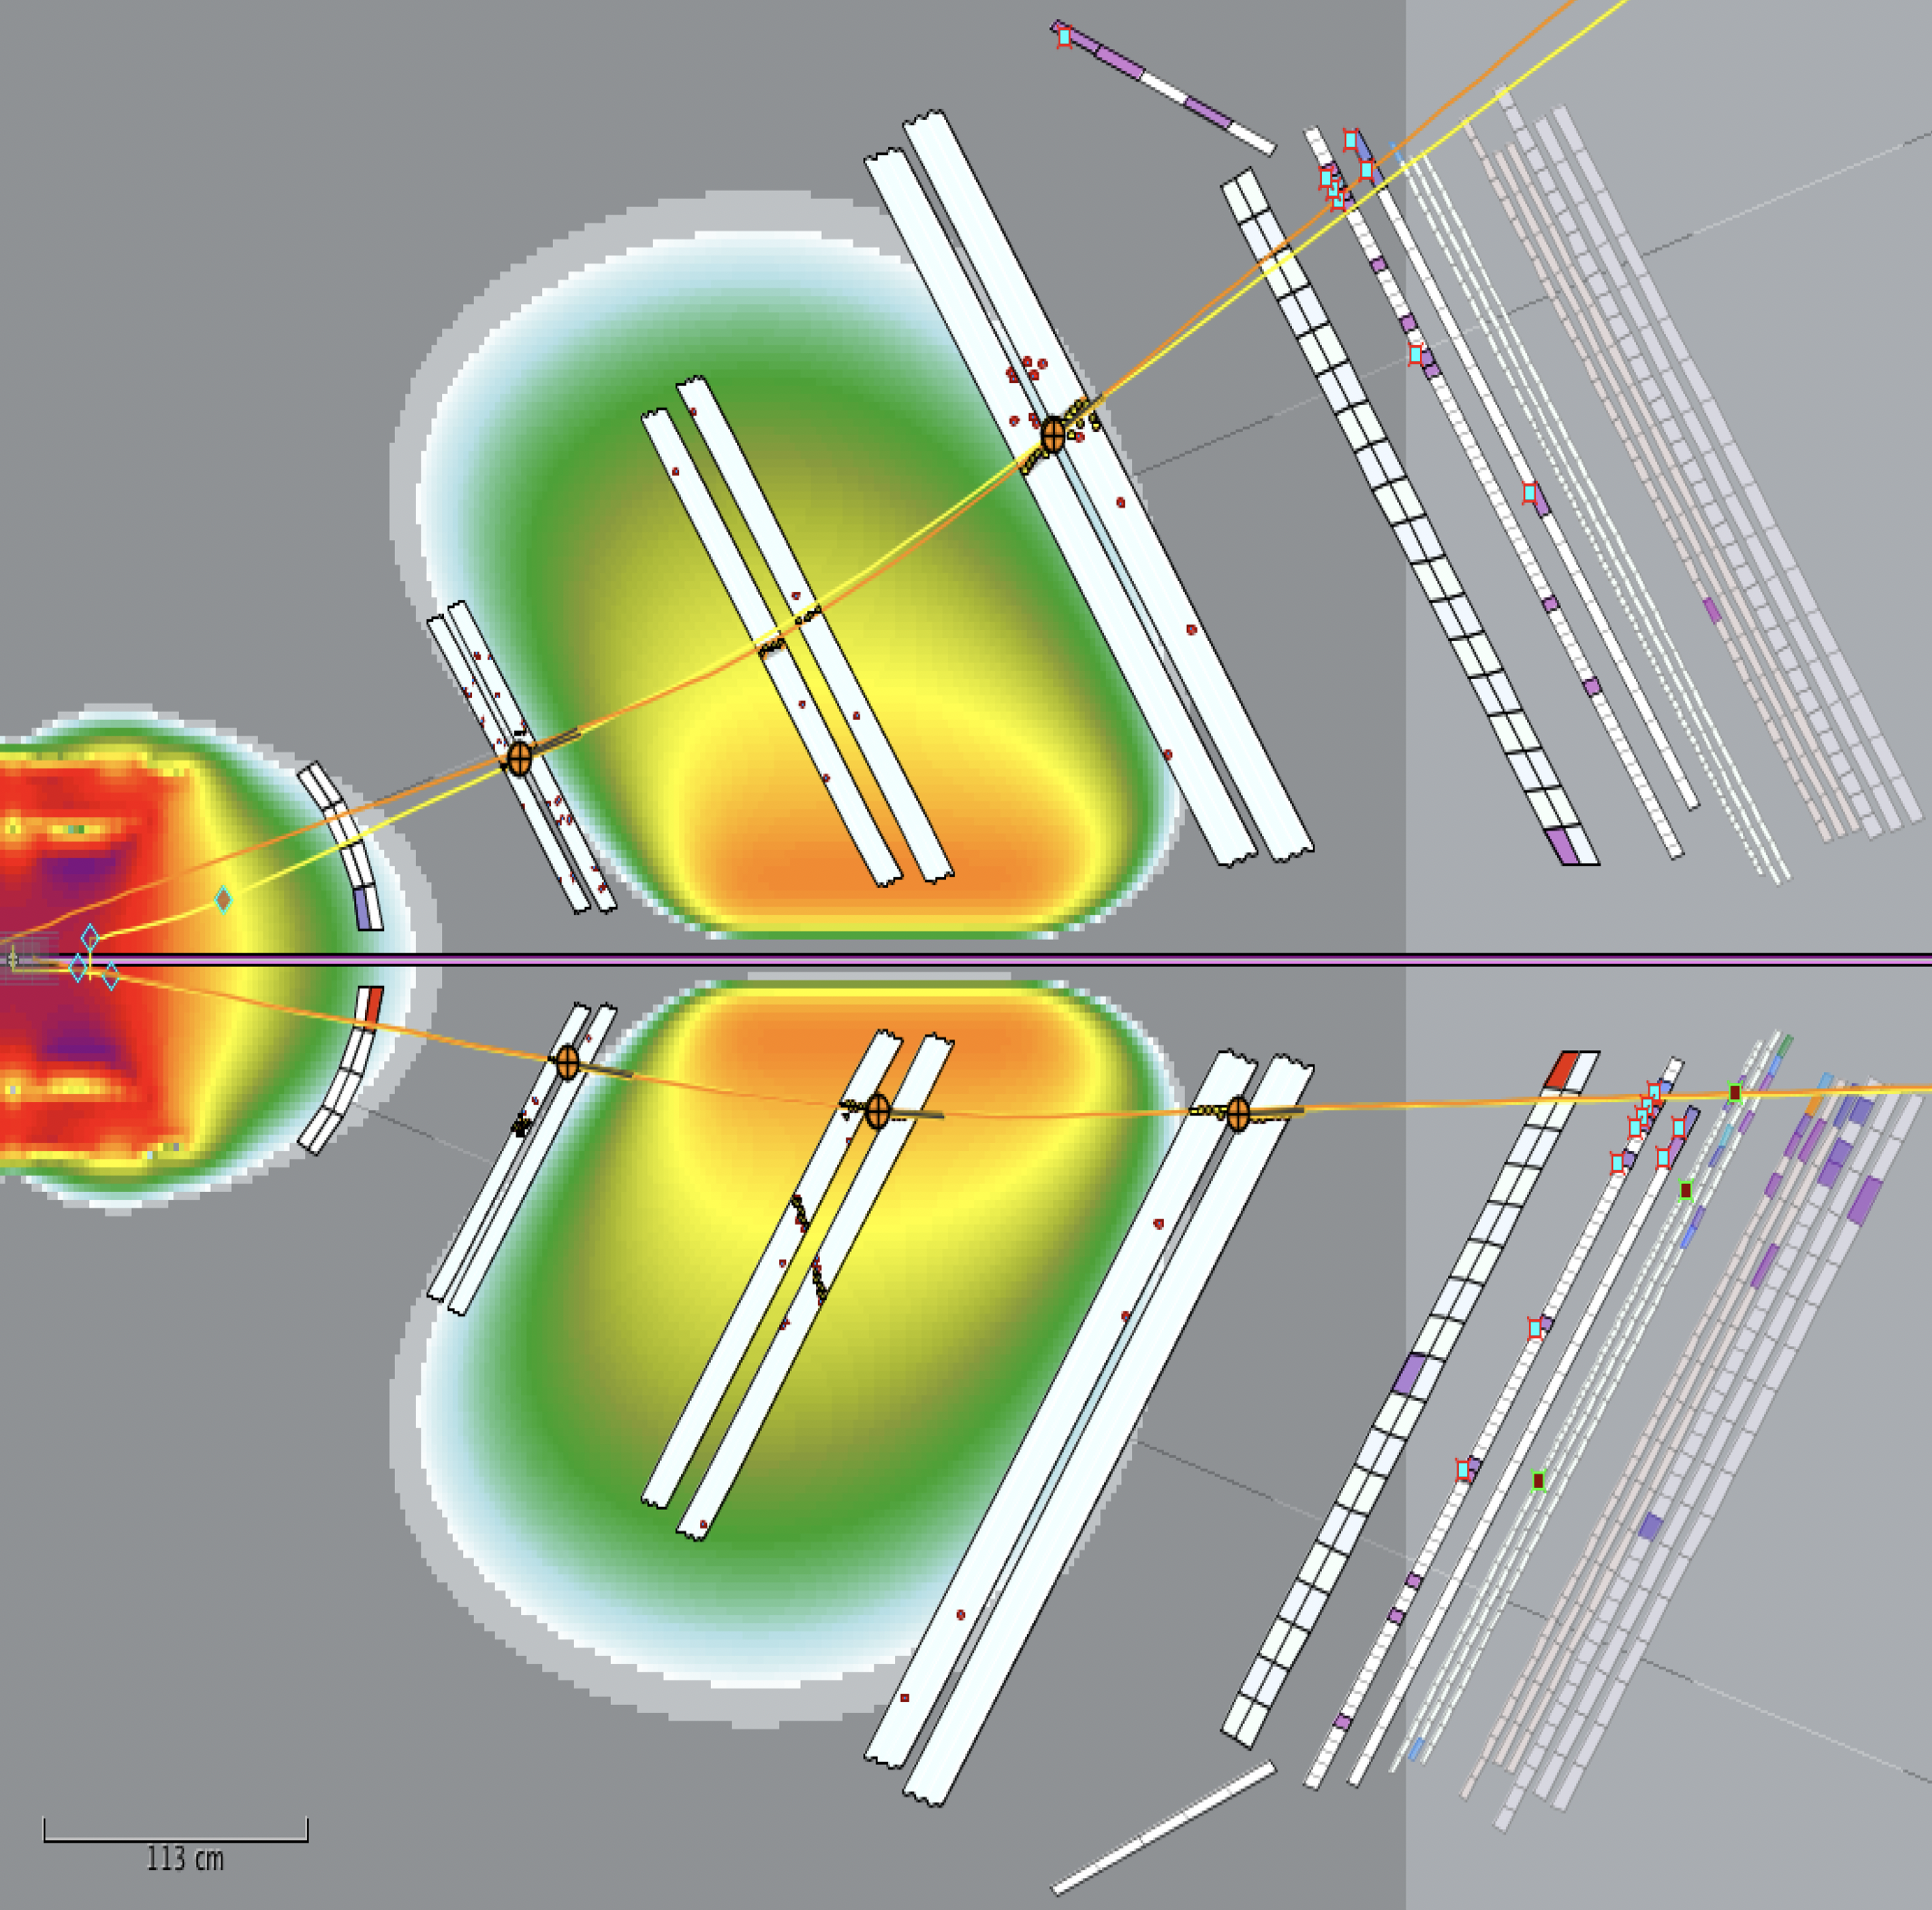
\includegraphics[width=1.0\columnwidth,keepaspectratio]{img/ced.png}
	\caption{CED Event Example}
	\label{fig:ced}
\end{figure}

\section{Network (Sergey)}

CLAS12 network is shown on Fig.~\ref{fig:network_diagram}. Its main component is Arista router serving as backbone for entire system. Set of main DAQ servers connected directly to that router by 40Gbit links. Some front-end components with high data rate connected directly to the router by 10Gbit links. Most of front-end conponents, as well as workstations are connected to the network switches using 1Gbit links, while those switches are connected to the router by 10Gbit links. Two 40Gbit uplinks connects entire system to the JLAB computer center.

Most of 1Gbit links uing copper wires while 10Gbit and 40Gbit ones using optic fibers, with the exception of short range server links where 40Gbit wires are used.

CLAS12 network shows adequate performance and high level of reliability. With projected data rates, it can be used 'as is' for the number of years.

\begin{figure}[hbt]
	\centering
	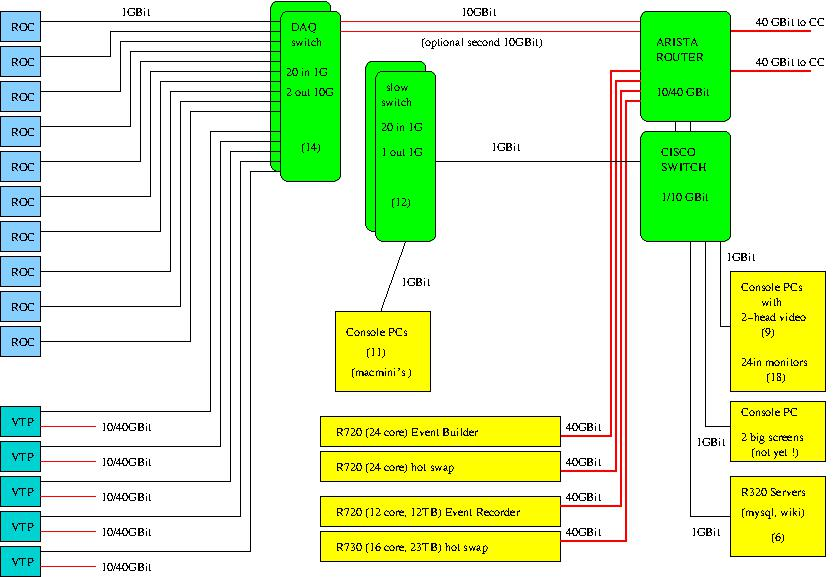
\includegraphics[width=1.0\columnwidth,keepaspectratio]{img/CLAS12_NET_1.jpg}
	\caption{CLAS12 DAQ Network Diagram}
	\label{fig:network_diagram}
\end{figure}

\section{Slow Controls}

The CLAS12 slow controls system was heavily upgraded for the 12 GeV era at JLab.  It incorporates legacy and modern hardware and standalone controls systems into full EPICS integration, such that everything is accessible from a single interface and on any computer in the CLAS12 system.  Another important aspect is leveraging standard infrastructure tools supported by central JLab computing resources, for a manageable and reliable controls system.

The CLAS12 slow controls system is based on Experimental Physics Industrial Control System (EPICS), currently version 3.14.12.5 \cite{epics-website}, and includes about 100 EPICS input-output controllers (IOCs) interfacing with approximately 50 different types of hardware via various communication protocols and over 800K process variables (PVs).

The controls system monitors and controls all aspects of the CLAS12 detector, beamline, and magnet systems, with monitoring on the DAQ system.  This includes power supplies from a variety of manufacturers, programmable logic controllers, cryogenic and gas systems, multiple scaler hardware, flasher sytems, all of the VXS crates, trigger system performance, and beamline motors, with sequencing for more complex operations like polarimetry and magnet hystereses.  An example of the superconducting torus magnet nitrogen system and 10~kHz EPICS monitoring is shown in Fig.~\ref{fig:tordaq}, and one of the scaler displays covering multiple CLAS12 detector systems is shown in Fig.~\ref{fig:jlabscalers}.

\begin{figure}[htbp]\centering
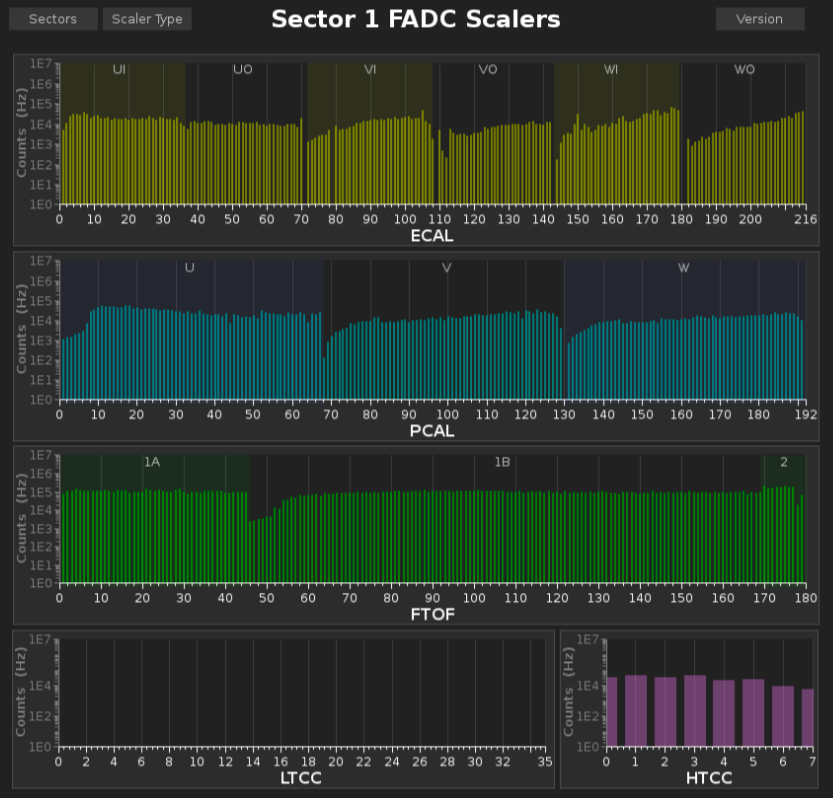
\includegraphics[width=8cm]{img/fd-scalers}
\caption{An example of the JLab FADC250 scalers for the CLAS12 PMT-based detector systems.\label{fig:jlabscalers}}
\end{figure}

\begin{figure*}[t]\centering
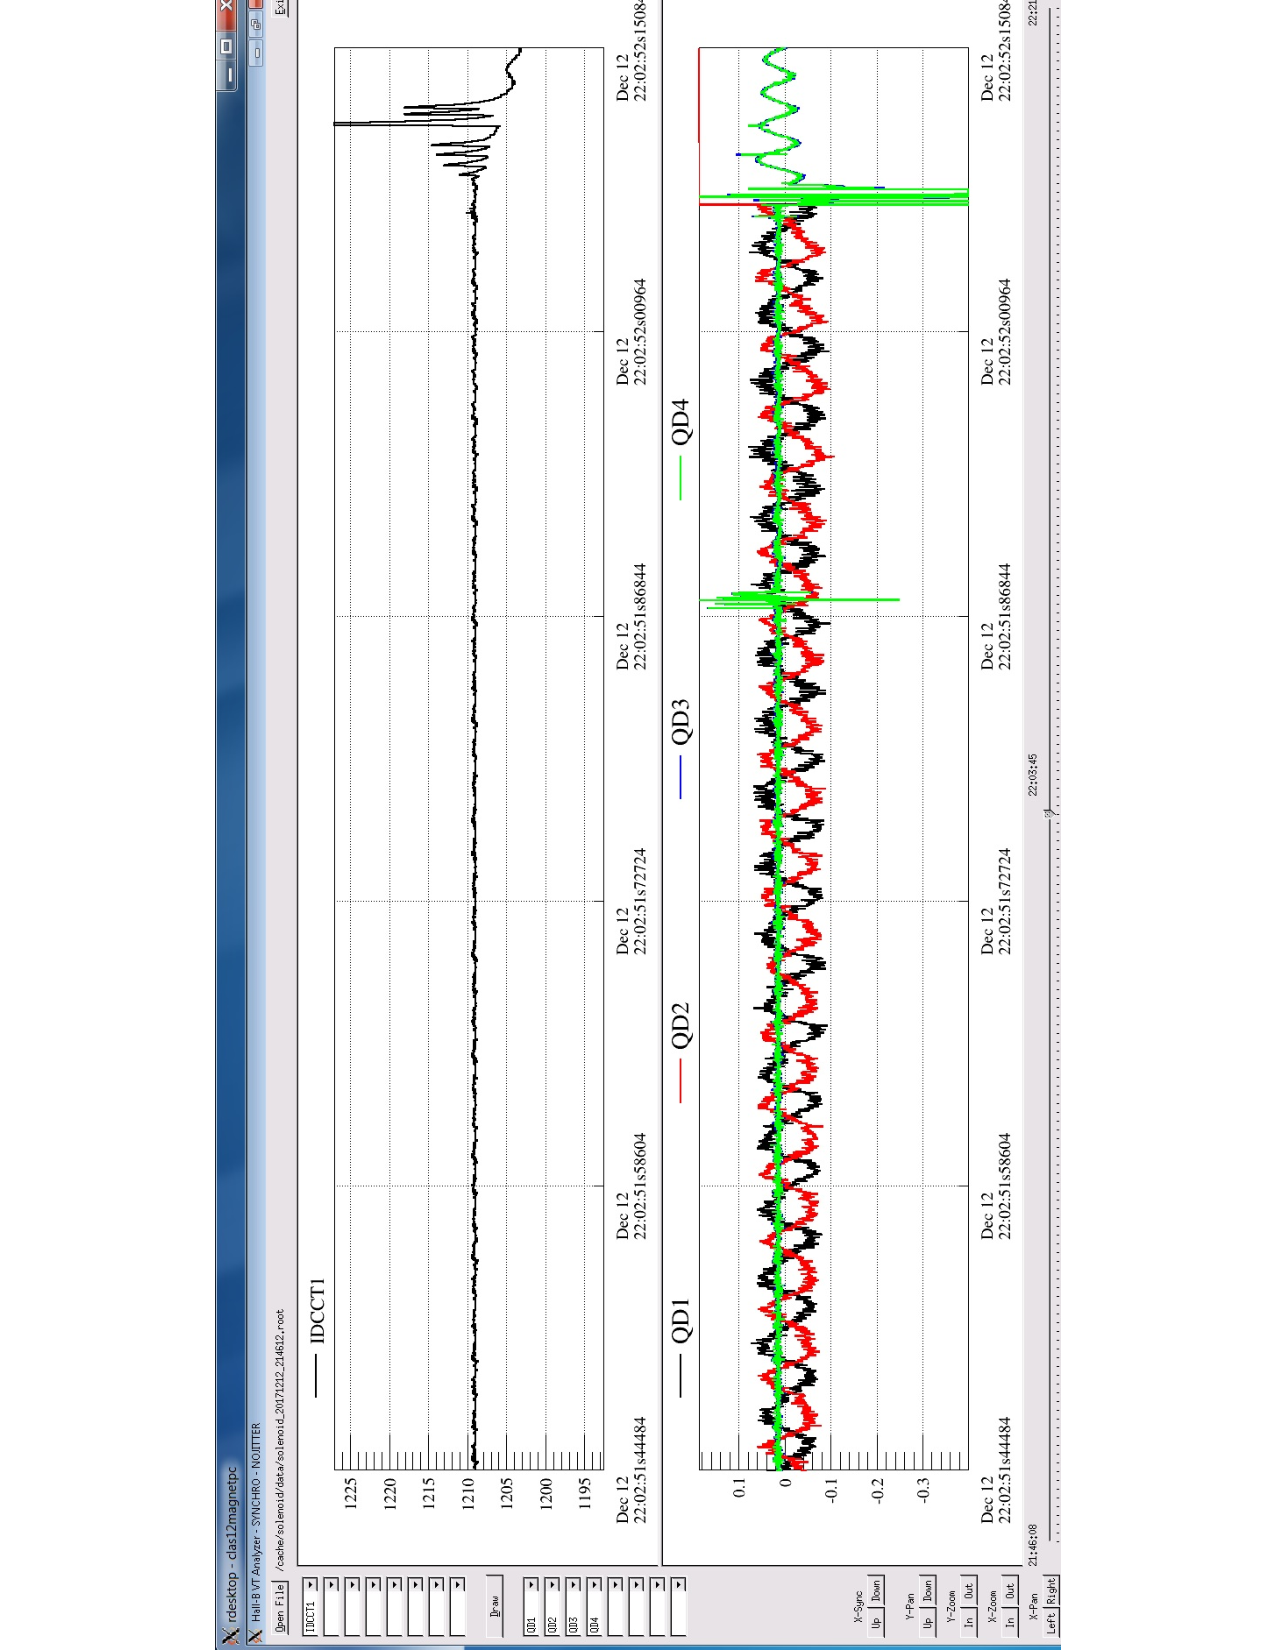
\includegraphics[width=0.9\textwidth]{img/tordaq}
\caption{The 10 kHz EPICS-based readout of the superconducting magnet quench detection system.\label{fig:tordaq}}
\end{figure*}

Most of the IOCs run on standard rack-mounted servers running Red Hat Enterprise 7 (RHEL7) in the Control Room.  A few IOCs run in more specialized systems in the experimental hall, such as VxWorks 5.X real-time operating systems on Motorolla VME controllers, primarily for high-rate, synchronous beam monitoring and support of legacy components.  All IOCs and associated processes are managed with procServ for interactive access when necessary and cronjobs for automatic startup and recovery \cite{procserv-website}.

For the graphical user interface we chose the modern Control Systems Studio (CS-Studio) developed at Oak Ridge National Laboratory \cite{css-website}.   CS-Studio is an Eclipse-based suite of tools for developing and monitoring large-scale control systems.  It includes various features supporting quick interface development, such as templating and dynamic generation.

We also use the CS-Studio alarm system.  It is based on a MYSQL database for storing alarm configurations, status, and message history, combined with a server monitoring the IOCs, updating the database, and communicating with clients.  The clients include a graphical interface tightly integrated with the rest of the controls system, with visible feedback and heirarchical view of the alarm system, an annuciator service running in the background in the Control Room, and a notifier service sending emails to on-call experts on particular alarm conditions.

Controls systems interfaces are all run locally on any desktop PC running RHEL7 in the Counting House.  Full remote access is also provided via 2-factor authentication and X-forwarding or VNC, as well as VMWare virtual machines supported by JLab.  Read-only access in a web browser is provided via WebOPI, another product affiliated with CS-Studio.

We utilize two internal EPICS channel access gateways, one read-only for the web interface, and the other for minimizing connections to superconducting magnet controls systems.  Wherever appropriate, the standard autosave feature of EPICS is utilized to automatically preserve settings across IOC reboots, and the standard Burt save/restore mechanisms.  The controls system also utilizes many custom hardware and software interlocks.

An important component of the slow controls system is archiving data.  For this we utilize the EPICS archiving system called Mya, a product developed by and in support of accelerator operations at JLab and shared with the experimental halls.  This provides storage and access to many previous years data of all CLAS12 EPICS PVs \cite{mya}.

Installation and configuration of the associated desktop and server machines, including custom service daemons, cron jobs, IOCs, network disk mounting, and deployment of upgrades and software changes, is managed via puppet and a central server maintained by JLab \cite{puppet-website}. The resulting maintainence is almost hands-free, and recovery from hardware failures or power outages is largely automated.  Monitoring of the servers is performed with Nagios, also provided by JLab, which provides email notifications about system errors \cite{nagios-website}.


\section{Performance}The HTCC is one of the major CLAS12 systems used in experiments with the electron beam. The most important aspects of the HTCC performance are that it provides good timing, high electron detection efficiency, high signal strength, and high rejection factor of charged pions. All these parameters are critical for the quality of the data obtained in experiments since the detector, in combination with the forward calorimeter [ref. to ECAL], provides a fast trigger signal for CLAS12. As shown in section 6 the MC prediction for the HTCC for electrons is $\approx$100\%. Fig.~\ref{fig:RAFO_2GeV}. shows the experimentally measured electron detection efficiency for elastically scattered electrons at 2 GeV. The corresponding thresholds applied were approximately 2.5 photoelectrons. Measurements were performed using a special procedure with a random trigger that was not correlated with the HTCC. There were observed 27 events not detected by the HTCC due to the applied threshold. As shown, the electron detection efficiency is $\eta$ = (99$\pm$0.2)\%, which is in good agreement with the MC estimate. This result can be considered as a conservative estimate due to relatively high threshold used in measurements. Moreover, electrons travel a longer distance in the radiator gas (10 \% to 30 \% difference depending on a scattering angle). For these electrons the signal strength is higher, and therefore the detection efficiency is higher also as compared with the aforementioned efficiency for the elastically scattered electrons.   

\begin{figure}[!ht]
    \centering
    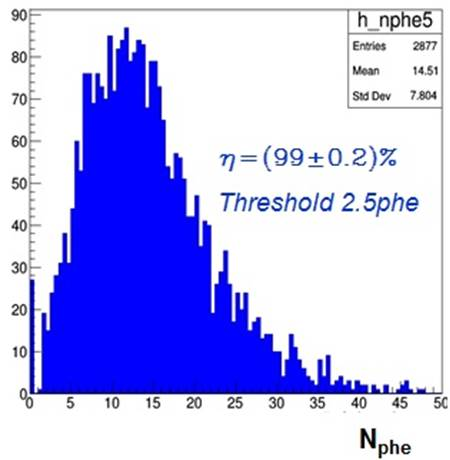
\includegraphics[width=1.0\linewidth,trim={0.0cm 0.0cm 0.0cm 0.0cm},clip]{images/RAFO_2GeV.jpg}
    \caption{Electron detection efficiency for elastically scattered electrons at 2 GeV. Data are obtained with the random trigger not correlated with the HTCC or other detector components of CLAS12.}
    \label{fig:RAFO_2GeV}
\end{figure}

Fig.~\ref{fig:positivePNPEC6595} shows the response of the detector in a wide range of particle momentum. The increase of number of events at high momenta is due to registration of charged pions (above threshold of their registration in the HTCC) and this is clearly illustrated.

\begin{figure}[!ht]
    \centering
    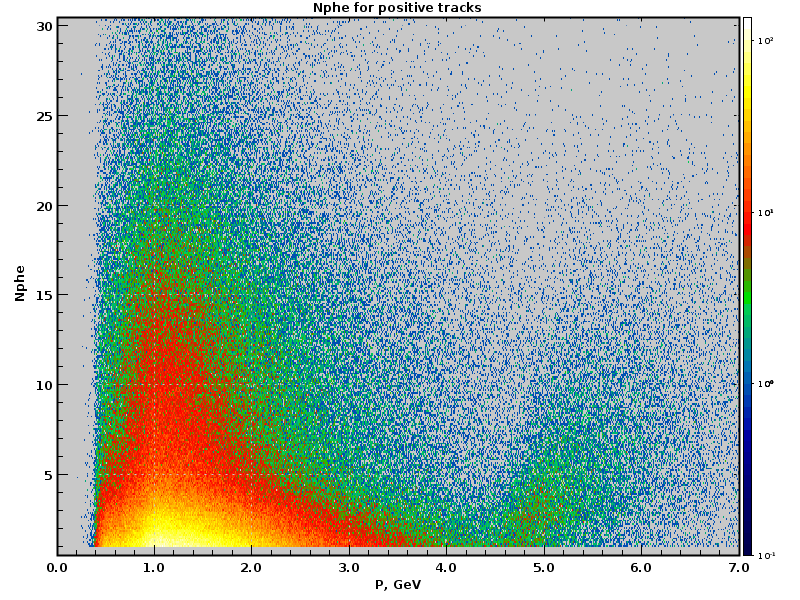
\includegraphics[width=1.0\linewidth,trim={0.0cm 0.0cm 0.0cm 0.0cm},clip]{images/positivePNPEC6595.png}
    \caption{Distributions of the HTCC response in a wide momentum range, including the region beyond the threshold of charged pion registration. Data obtained for positrons and $\pi^{+}$-mesons.}
    \label{fig:positivePNPEC6595}
\end{figure}

\begin{comment}
As shown bellow in the Fig.~\ref{fig:avgNPE_Theta_Phi_Dev_Build-2_NO_HOLES} the signal strength goes up for the utmost mirrors (large electron scattering angles). This is because electrons travel a longer distance in the radiator gas (10\% to 30\% difference depending on angle.) In other words the electron detection efficiency obtained for elastically scattered electrons at 2 GeV can be considered as as a conservative estimate for the efficiency of electron detection at larger angles.
\end{comment} 

The signal strength in the HTCC depends on the actual properties of the mirror facets, such as their final shape and reflectance. The accuracy of the combined mirror assembly and the alignment of the HTCC components (mirror, PMTs, Winston Cones), and the composition of the radiator gas all influence the final results. The FADC histogram of  the typical signal strength distribution obtained in one half-sector \#1 and \#2 of Sector 1 is shown in Fig.~\ref{fig:Signal_S1_HS1_HS2_R1_R2}. The signal strength for scattered electrons averaged over all HTCC channels is shown in Fig.~\ref{fig:Average_HTCC_Signal}. The experimentally measured mean value of 16.3 phe is close to Monte-Carlo simulation results, (see Fig.~\ref{fig:10cm_Targ_5T_Field_Phi}).

\begin{figure}[!ht]
    \centering
    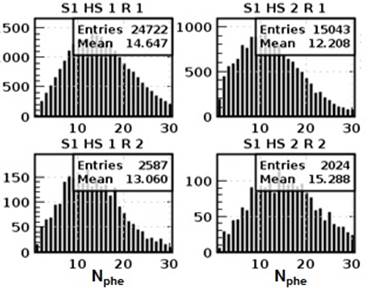
\includegraphics[width=1.0\linewidth,trim={0.0cm 0.0cm 0.0cm 0.0cm},clip]{images/Signal_S1_HS1_HS2_R1_R2.jpg}
    \caption{Typical distributions of the signal strength in channels covering polar angles in the range of $5^\circ$ to $12.5^\circ$ (Ring 1) and $12.5^\circ$ to $20.0^\circ$ (Ring 2) within azimuthal interval of $60^\circ$.}
    \label{fig:Signal_S1_HS1_HS2_R1_R2}
\end{figure}

\begin{figure}[!ht]
    \centering
    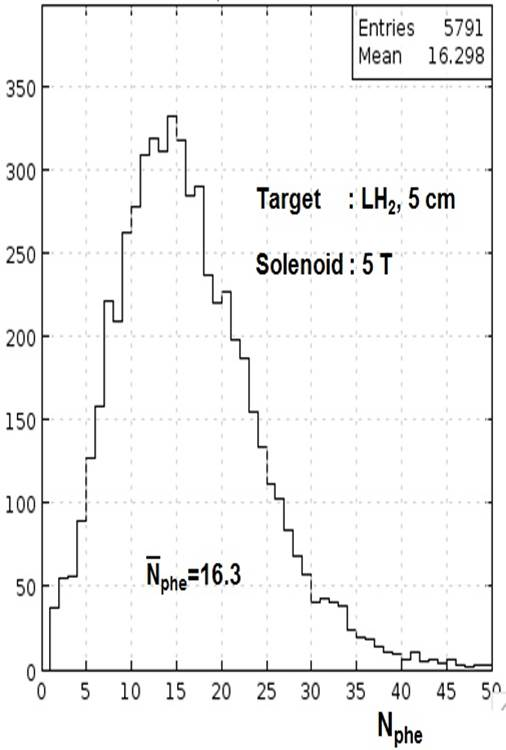
\includegraphics[width=1.0\linewidth,trim={0.0cm 0.0cm 0.0cm 0.0cm},clip]{images/Average_HTCC_Signal.jpg}
    \caption{The HTCC average signal strength for electrons from beam data.}
    \label{fig:Average_HTCC_Signal}
\end{figure}

Fig.~\ref{fig:HTCC_Response_run4013} shows the HTCC response for different electron momenta. Fig.~\ref{fig:avgNPE_Theta_Phi_Dev_Build-2_NO_HOLES}  shows the distribution of the HTCC response over the entire face of the mirror in the $x-y$-plane. Similar distribution is shown in Fig.~\ref{fig:avgNPE_XY_Dev_Build_02npe} obtained at the lower electron detection threshold of 0.2 photoelectrons. At the large electron scattering angles in range of 27.5$^\circ$ to 35$^\circ$, the statistics is lower. Fig.~\ref{fig:statistics_Theta_Phi_Dev_Build_NO_HOLES} shows the distribution of statistics in all 6 sectors. The data shows that the integrated signal strength is about 16.5 photoelectrons.

\begin{figure}[!ht]
    \centering
    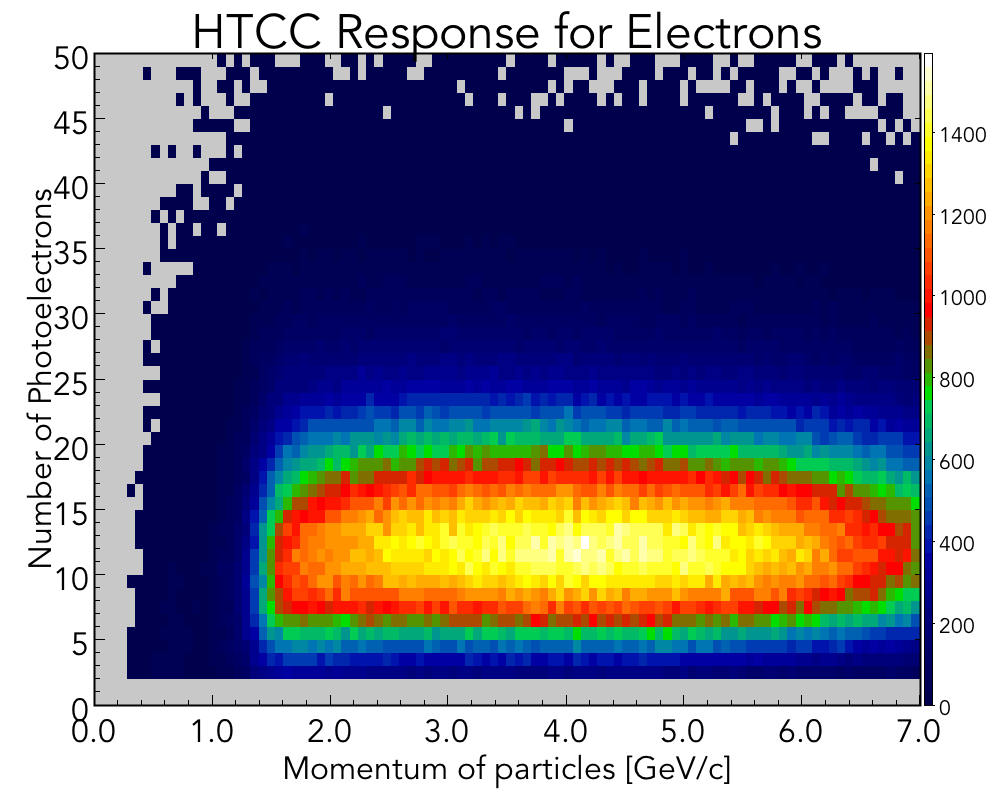
\includegraphics[width=1.0\linewidth,trim={0.0cm 0.0cm 0.0cm 1.73cm},clip]{images/HTCC_Response_run4013.png}
    \caption{The HTCC response for electrons: signal strength vs. momentum at 10.6 GeV energy.}
    \label{fig:HTCC_Response_run4013}
\end{figure}

\begin{figure}[!ht]
    \centering
    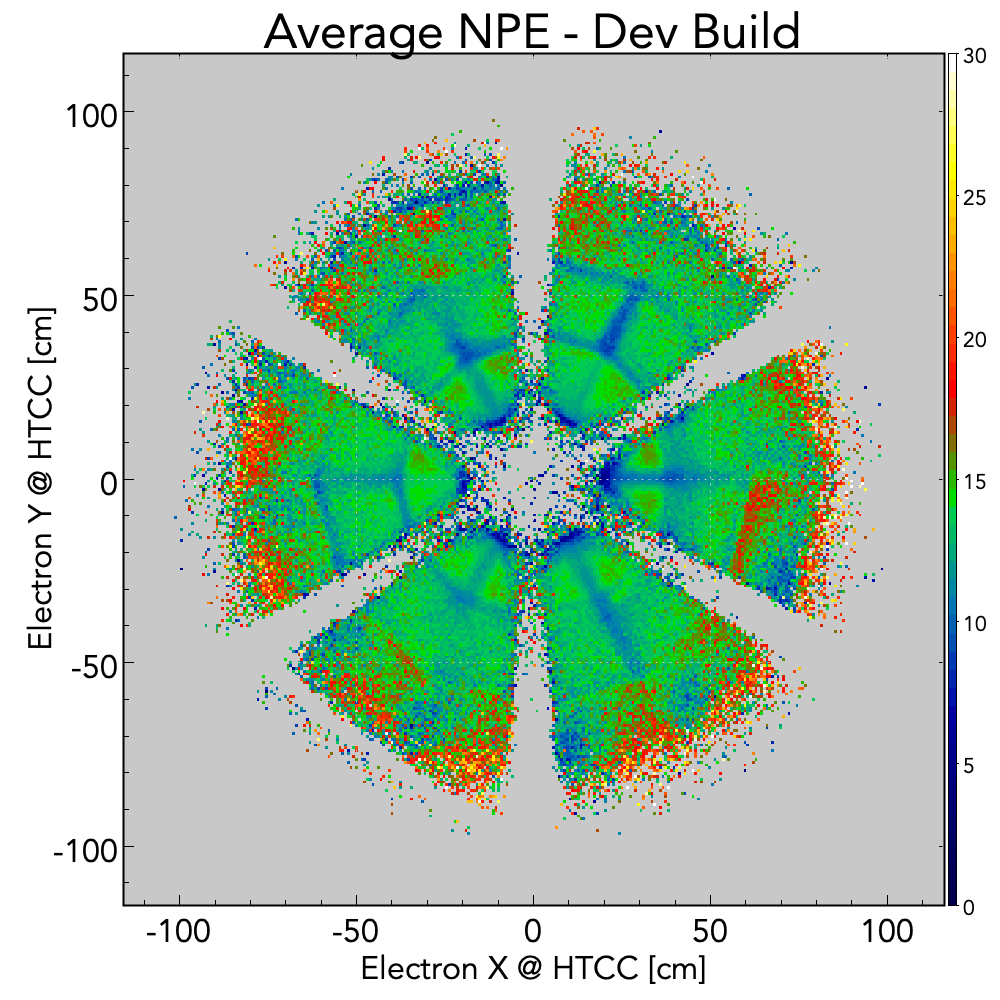
\includegraphics[width=1.0\linewidth,trim={0.0cm 0.0cm 0.0cm 1.67cm},clip]{images/avgNPE_Theta_Phi_Dev_Build-2_NO_HOLES.png}
    \caption{The HTCC response (in $N_{phe}$) for electrons in $x-y$-plane of the mirror.}
    \label{fig:avgNPE_Theta_Phi_Dev_Build-2_NO_HOLES}
\end{figure}

\begin{figure}[!ht]
    \centering
    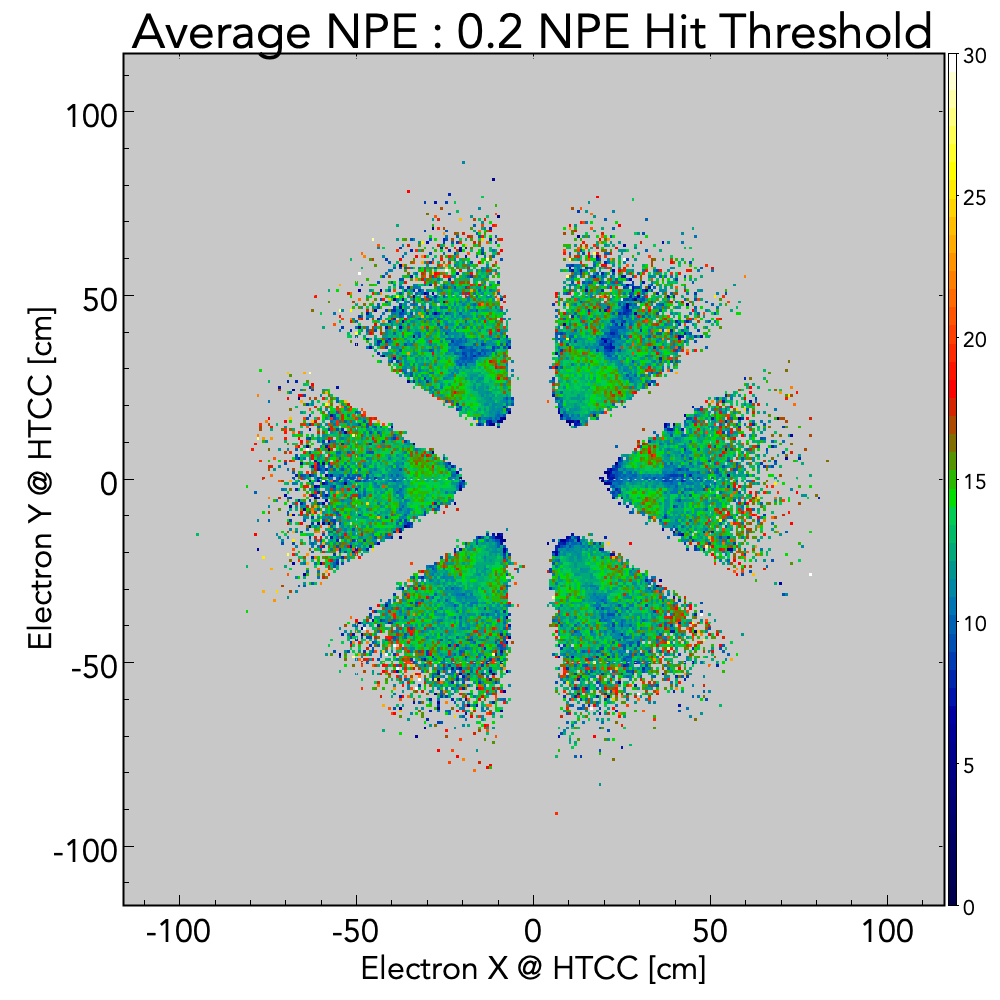
\includegraphics[width=1.0\linewidth,trim={0.0cm 0.0cm 0.0cm 1.67cm},clip]{images/avgNPE_XY_Dev_Build_02npe.png}
    \caption{The HTCC response (in $N_{phe}$) for electrons in $x-y$-plane of the mirror at the electron detection threshold of 0.2 photoelectrons.}
    \label{fig:avgNPE_XY_Dev_Build_02npe}
\end{figure}

\begin{figure}[!ht]
    \centering
    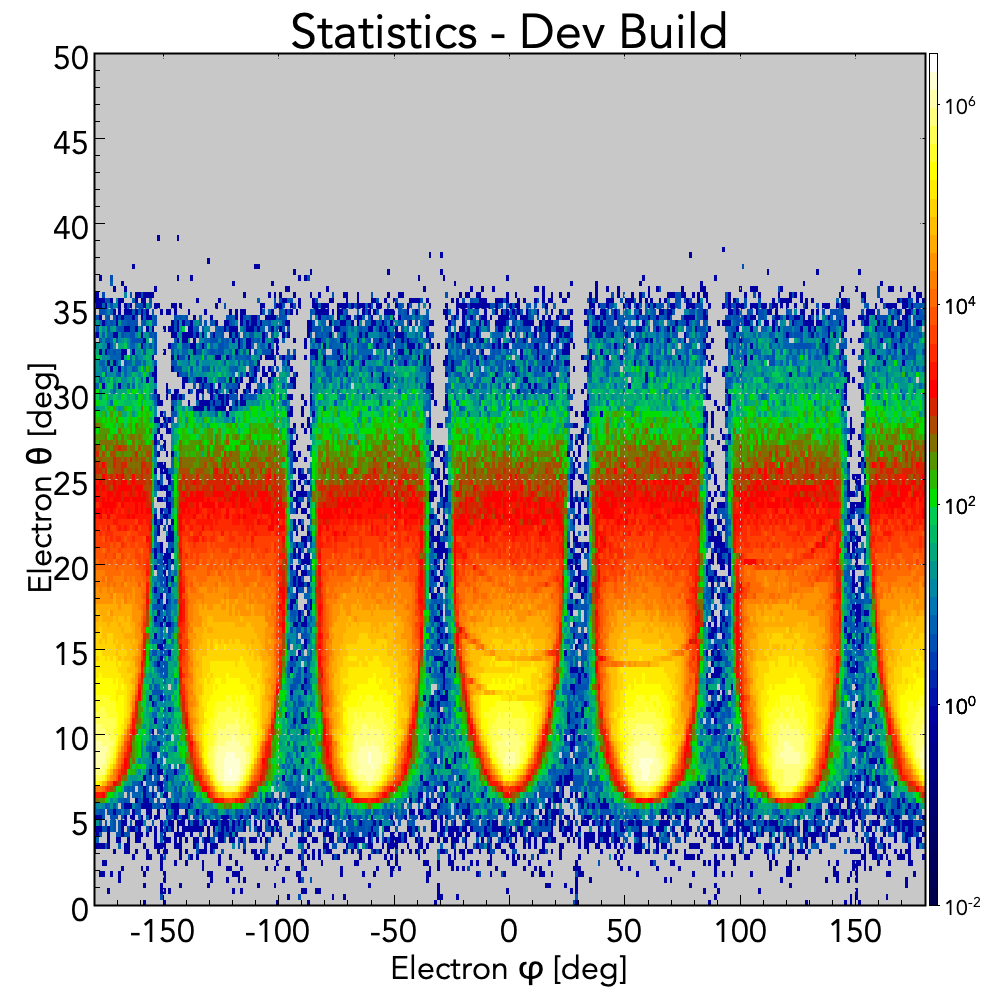
\includegraphics[width=1.0\linewidth,trim={0.0cm 0.0cm 0.0cm 1.67cm},clip]{images/statistics_Theta_Phi_Dev_Build_NO_HOLES.png}
    \caption{Distribution of statistics in all 6 sectors.}
    \label{fig:statistics_Theta_Phi_Dev_Build_NO_HOLES}
\end{figure}

We also note that in cases when the electrons cross the mirror close to its edges (at approximately at 5$^\circ$ and 35$^\circ$) one should expect unavoidable losses in the signal strength: some part of the Cherenkov light just passes by the mirror. As far as the internal borders between adjacent mirrors are concerned, there are similar losses that take place and are finally partially compensated due to the complete azimuthal symmetry of the detector, see Fig.~\ref{fig:avgNPE_Theta_Phi_Dev_Build-2_NO_HOLES}. The width of that area along internal boundaries that is deformed in the direction normal to the mirror face due to the shrinkage of the glue is estimated between $\sim$5 to $\sim$10 mm. This area includes the technological zone ~0.5 mm of width that is not reflecting the light at all. As a result these regions (width up to $\sim$10 mm) along internal boundaries between mirror facets defuse the light impinging the area, and therefore the signal strength is reduced. this edge effect is normal for the given design of the detector.


\section{Acknowledgements}

We appreciate the contribution of J.  Andresen, C. Britton, S. Chappa, A. Dyer, J. Hoff, V. Re, and T. Zimmerman to the design of the HFCB. We are grateful to administrative, engineering, and technical staff of Fermilab Silicon Detector Facility for excellent work on module assembly.

\section{Conclusions}

The SVT is installed in the CLAS experimental hall, performance of modules measured during detector integration has been confirmed. No channels were lost during the installation. SVT barrel has been electrically  tested with number of defective channels 0.1$\%$, well within the specification. The chip average ENC noise is uniform $\sim$1600 e in normal operating conditions. There is no evidence of coherent noise between the modules and other components. The tracker has been commissioned with cosmic rays and integrated as part of  CLAS central detector. Tracking performance was confirmed with beam data and matches physics requirements. 





\section{References}

%%\bibliography{bibfile}
%%\bibliographystyle{elsarticle-num}

\begin{thebibliography}{99}

	\bibitem{clas-nim}
	B.A. Mecking {\it et al.}, Nucl. Inst. and Meth. {\bf A503}, 513 (2003).
	
	\bibitem{tcs-ref}
	XXX {\it et al.}, {\it ``The YYY Boards''}.
	
	\bibitem{ti-ref}
	XXX {\it et al.}, {\it ``The TI Board''}.

	\bibitem{td-ref}
	XXX {\it et al.}, {\it ``The TD Board''}.

	\bibitem{ts-ref}
	XXX {\it et al.}, {\it ``The TS Board''}.

	\bibitem{sd-ref}
	XXX {\it et al.}, {\it ``The SD Board''}.

	\bibitem{fadc-ref}
	XXX {\it et al.}, {\it ``The FADC Board''}.

	\bibitem{dsc2-ref}
	XXX {\it et al.}, {\it ``The DSC2 Board''}.

	\bibitem{dcrb-ref}
	XXX {\it et al.}, {\it ``The DCRB Board''}.

	\bibitem{vscm-ref}
	XXX {\it et al.}, {\it ``The VSCM Board''}.

	\bibitem{tdc-ref}
	XXX {\it et al.}, {\it ``The TDC Board''}.

	\bibitem{ssp-ref}
	XXX {\it et al.}, {\it ``The SSP Board''}.

	\bibitem{coda-ref}
	XXX {\it et al.}, {\it ``The CODA System'}.

	\bibitem{svt-ref}
	XXX {\it et al.}, {\it ``The CLAS12 SVT Detector'}, see this issue.

	\bibitem{trig-ref}
	B.Raydo {\it et al.}, {\it ``The CLAS12 Trigger System'}, see this issue.

\end{thebibliography}

\end{document}








